% =============================================================================
% InstructorHandouts/CS301/01-foundations-pointers-adt-instructor-handout.tex
% Instructor Handout 1: Where Does Your Data Live?
%
% INSTRUCTOR-ONLY. Complete, self-contained teaching guide -- explanation,
% embedded diagrams, presentation guidance, and delivery commentary are woven
% together per topic (not split into separate documents/sections), so an
% instructor can teach directly from this file with no slides or Notes open.
% Explanations/diagrams/examples trace to Slides/CS301/01-foundations-pointers-adt.tex
% and Notes/CS301/01-foundations-pointers-adt-notes.tex; "Teaching note"
% asides are instructor judgment, visually distinguished but not a separate
% section.
%
% FULL REGENERATION 2026-08-13: the deck was rebuilt at --difficulty intro
% (course-wide default change, knowledge-base-CS301.md) and gained real
% content relative to the prior core-tier deck this handout was originally
% built from: a new standalone Act 0 (motivation/roadmap/running thread), a
% new "Structured Programming" Act (three control patterns + worked example),
% and the full malloc/calloc/realloc/free family inside "One Heap Block"
% (the prior deck deferred calloc/realloc entirely -- that scope notice is
% now WRONG and has been removed). This is a full regeneration, not a patch
% on the prior core-tier handout.
%
% Board-Drawable Example standard (see .claude/skills/instructor-handout/SKILL.md):
% every topic with worked content carries >=2 distinct board-drawable examples,
% each with an explicit board build order; each is marked "Board:" plus a
% live-interaction hook.
%
% Figure policy (user directive, 2026-08-13): every deck TikZ diagram that
% this handout walks through is reused VERBATIM from
% Slides/CS301/01-foundations-pointers-adt.tex -- none re-derived, none
% omitted. The strict TikZ P7 zero-overlap audit is relaxed for this
% print/study artifact (minor sub-cm label/line proximity is tolerable here);
% only a full obscure or a path running through a box would be fixed.
%
% Page-verified anchors (per knowledge-base-CS301.md):
%   Wirth2004 Sec4.1 p.109 (motivation), Sec4.2 p.111 (pointer/dynamic
%   allocation). Sedgewick2011 Sec1.2 p.64 (ADT definition), Sec1.3 p.120
%   (bag/queue/stack collection types), Sec1.4 p.172 (cost-analysis
%   motivation). Karumanchi2017 Ch.1 pp.18-19 PDF (two-part ADT definition,
%   commonly-used-ADTs list) -- confirmed NOT a source for structured
%   programming or malloc/calloc/realloc/free (Step 0.5 coverage check).
%   Horowitz & Sahni Ch.1 and Aho-Hopcroft-Ullman Ch.1: chapter-level only,
%   not yet page-indexed. calloc/realloc and structured programming carry no
%   textbook citation in the deck itself, so none is invented here.
%
% Compile (Windows/MiKTeX, ';'-joined TEXINPUTS/BIBINPUTS): cd InstructorHandouts/CS301 &&
%   TEXINPUTS="../../Preambles;" xelatex -interaction=nonstopmode 01-foundations-pointers-adt-instructor-handout.tex
%   BIBINPUTS="../..;" bibtex 01-foundations-pointers-adt-instructor-handout
%   TEXINPUTS="../../Preambles;" xelatex -interaction=nonstopmode 01-foundations-pointers-adt-instructor-handout.tex  (x2)
% =============================================================================

\documentclass[11pt]{article}
\usepackage[margin=1in]{geometry}
% =============================================================================
% Preambles/header.tex — shared LaTeX/Beamer preamble for this project
%
% Use from a Beamer lecture by prepending:
%     % =============================================================================
% Preambles/header.tex — shared LaTeX/Beamer preamble for this project
%
% Use from a Beamer lecture by prepending:
%     % =============================================================================
% Preambles/header.tex — shared LaTeX/Beamer preamble for this project
%
% Use from a Beamer lecture by prepending:
%     \input{header}
% and compiling with TEXINPUTS=../Preambles:$TEXINPUTS (the /compile-latex
% skill does this automatically).
%
% PALETTE CONTRACT. Color names defined here MUST match the names in
% Quarto/theme-template.scss so Beamer and Quarto renderings use the same
% palette. The scripts/check-palette-sync.sh script enforces this.
%
% To customize: edit the HEX values below AND the matching $variable in
% Quarto/theme-template.scss, then run scripts/check-palette-sync.sh.
%
% TITLE PAGE. A formal, serif (Libertine) title-page template is defined in
% the Beamer-only block below (\setbeamertemplate{title page}) -- title,
% subtitle, a thin gold rule, then \author/\institute/\date. Frametitle and
% body text remain on Beamer's sans-serif default. No SCSS counterpart is
% needed for this (font/layout only, no new colors).
% =============================================================================

% -----------------------------------------------------------------------------
% Engine detection + encoding
%
% Our /compile-latex skill uses XeLaTeX, where inputenc is unnecessary and
% can produce encoding warnings. Only load inputenc under pdfTeX.
% -----------------------------------------------------------------------------
\usepackage{iftex}
\ifPDFTeX
  \usepackage[utf8]{inputenc}
\fi

\usepackage{amsmath, amssymb, amsthm}
\usepackage{booktabs}
\usepackage{graphicx}

% -----------------------------------------------------------------------------
% Serif face for the title page (formal/academic look). Linux Libertine is
% XeLaTeX- and pdfTeX-safe and redefines \rmdefault, so \rmfamily picks it up
% everywhere \rmfamily is used explicitly. Body text and frametitles stay on
% Beamer's own sans-serif default (unaffected) -- only the title-page
% \setbeamerfont{...} overrides below opt in to \rmfamily.
% -----------------------------------------------------------------------------
\usepackage{libertine}

% -----------------------------------------------------------------------------
% PALETTE — mirrors Quarto/theme-template.scss variable names.
% Load xcolor and define colors BEFORE anything that references them
% (notably hyperref, hypersetup, and the Beamer color assignments).
% -----------------------------------------------------------------------------
\usepackage{xcolor}

\definecolor{primary-blue}{HTML}{012169}      % headings, accents
\definecolor{primary-gold}{HTML}{B9975B}      % emphasis, borders
\definecolor{highlight-yellow}{HTML}{F2A900}  % markers, alerts
\definecolor{light-bg}{HTML}{E8EDF5}          % title / section backgrounds
\definecolor{jet}{HTML}{1A1A1A}               % body text

% Semantic colors (used in diagrams and annotations)
\definecolor{positive}{HTML}{15803D}          % good / observed / identified
\definecolor{negative}{HTML}{B91C1C}          % bad / problematic / bias
\definecolor{neutral}{HTML}{525252}           % reference / context

% Highlight accents (match .hi-* classes in the SCSS)
\definecolor{hi-slate}{HTML}{314F4F}
\definecolor{hi-green}{HTML}{2E8B57}
\definecolor{hi-red}{HTML}{C41E3A}

% Semantic aliases so skill templates and snippets can write
% \textcolor{accent}{...} without hard-coding "primary-blue".
\colorlet{accent}{primary-blue}
\colorlet{accent2}{primary-gold}

% -----------------------------------------------------------------------------
% Hyperref — loaded AFTER xcolor + palette so link colors resolve.
% -----------------------------------------------------------------------------
\usepackage{hyperref}
\hypersetup{colorlinks=true, linkcolor=primary-blue, urlcolor=primary-blue,
            citecolor=primary-blue, pdfborder={0 0 0}}

% -----------------------------------------------------------------------------
% Course code — set once per deck (after \input{header}, before \begin{document})
% via \coursecode{CS401}. Shown in the footer on every slide so a deck's course
% is identifiable without opening the title page. Empty by default.
% -----------------------------------------------------------------------------
\makeatletter
\newcommand{\coursecode}[1]{\gdef\@coursecodetext{#1}}
\gdef\@coursecodetext{}
\makeatother

% -----------------------------------------------------------------------------
% Beamer theme assignments (only apply under Beamer).
%
% We detect Beamer via \@ifclassloaded{beamer}, which is the documented,
% non-internal way. This must be wrapped in \makeatletter/\makeatother
% because \@ifclassloaded contains an @-catcode character.
% -----------------------------------------------------------------------------
\makeatletter
\@ifclassloaded{beamer}{%
  \usefonttheme{professionalfonts}
  \setbeamercolor{structure}{fg=primary-blue}
  \setbeamercolor{frametitle}{fg=primary-blue}
  \setbeamercolor{title}{fg=primary-blue}
  \setbeamercolor{subtitle}{fg=primary-gold}
  \setbeamercolor{author}{fg=primary-blue}
  \setbeamercolor{institute}{fg=neutral}
  \setbeamercolor{date}{fg=primary-gold}
  \setbeamercolor{itemize item}{fg=primary-blue}
  \setbeamercolor{itemize subitem}{fg=primary-gold}
  \setbeamercolor{alerted text}{fg=primary-gold}
  \setbeamercolor{block title}{fg=white, bg=primary-blue}
  \setbeamercolor{block body}{bg=light-bg}
  % Semantic block variants: block=definition/concept (blue), exampleblock=
  % worked example (green/positive), alertblock=key takeaway or caution (gold).
  % Keep to <=2 colored boxes per slide across ALL three variants (INV-7).
  \setbeamercolor{block title example}{fg=white, bg=positive}
  \setbeamercolor{block body example}{bg=light-bg}
  \setbeamercolor{block title alerted}{fg=white, bg=primary-gold}
  \setbeamercolor{block body alerted}{bg=light-bg}

  % ---------------------------------------------------------------------------
  % Formal title page: serif (Libertine, via \rmfamily) for title-page
  % elements only. Body text, itemize, and frametitle are intentionally left
  % on Beamer's sans-serif default -- \usebeamerfont{title} is also what
  % \transitionslide (below) uses for its big centered text, so section
  % transitions pick up the same serif treatment for free.
  % ---------------------------------------------------------------------------
  \setbeamerfont{title}{family=\rmfamily, series=\bfseries, size=\Large}
  \setbeamerfont{subtitle}{family=\rmfamily, shape=\itshape, size=\normalsize}
  \setbeamerfont{author}{family=\rmfamily, size=\normalsize}
  \setbeamerfont{institute}{family=\rmfamily, size=\scriptsize}
  \setbeamerfont{date}{family=\rmfamily, size=\scriptsize}

  \setbeamertemplate{title page}{
    \vfill
    \begin{center}
      {\usebeamerfont{title}\usebeamercolor[fg]{title}\inserttitle\par}
      \vspace{0.15cm}
      {\usebeamerfont{subtitle}\usebeamercolor[fg]{subtitle}\insertsubtitle\par}
      \vspace{0.45cm}
      {\color{primary-gold}\rule{0.42\textwidth}{0.6pt}\par}
      \vspace{0.45cm}
      {\usebeamerfont{author}\usebeamercolor[fg]{author}\insertauthor\par}
      \vspace{0.35cm}
      {\usebeamerfont{institute}\usebeamercolor[fg]{institute}\insertinstitute\par}
      \vspace{0.35cm}
      {\usebeamerfont{date}\usebeamercolor[fg]{date}\insertdate\par}
    \end{center}
    \vfill
  }

  % Minimal footer: course code (left) + page X / N (right), no navigation clutter
  \setbeamertemplate{navigation symbols}{}
  \setbeamertemplate{footline}{%
    \color{neutral}\footnotesize\hspace{0.7em}\@coursecodetext\hfill
    \insertframenumber/\inserttotalframenumber\hspace{0.7em}\vspace{0.3em}}
}{}
\makeatother

% -----------------------------------------------------------------------------
% TikZ setup — libraries the snippet gallery uses
% -----------------------------------------------------------------------------
\usepackage{tikz}
\usetikzlibrary{arrows.meta, positioning, calc, decorations.pathreplacing,
                fit, shapes.geometric, backgrounds}

% Shared TikZ styles — snippets and hand-written diagrams can pick these up
% via `\begin{tikzpicture}[every node/.style={...}]` or by naming specific
% styles (e.g., `\node[dag-node] (X) at (0,0) {X};`).
\tikzset{
  % Node styles for causal DAGs and similar
  dag-node/.style = {
    draw=primary-blue, fill=light-bg, rounded corners=2pt,
    minimum width=1.2cm, minimum height=0.9cm, align=center, font=\small
  },
  decision-node/.style = {
    draw=primary-gold, fill=white, diamond, aspect=1.8,
    minimum width=1.8cm, minimum height=1.2cm, align=center, font=\small,
    inner sep=1pt
  },
  % Edge styles — observed vs counterfactual
  observed-edge/.style = {-{Latex[length=2.5mm]}, thick, draw=jet},
  counterfactual-edge/.style = {-{Latex[length=2.5mm]}, thick, draw=neutral, dashed},
  confound-edge/.style = {-{Latex[length=2.5mm]}, thick, draw=negative, dashed},
  % Data-point styles for plots
  observed-dot/.style = {fill=primary-blue, draw=primary-blue, circle, inner sep=1.2pt},
  counterfactual-dot/.style = {fill=white, draw=neutral, circle, inner sep=1.2pt}
}

% -----------------------------------------------------------------------------
% Convenience macros
% -----------------------------------------------------------------------------
\newcommand{\muted}[1]{\textcolor{neutral}{#1}}
\newcommand{\key}[1]{\textcolor{primary-gold}{\textbf{#1}}}
\newcommand{\good}[1]{\textcolor{positive}{#1}}
\newcommand{\bad}[1]{\textcolor{negative}{#1}}

% Standout frame macro: full-bleed dark background for section transitions.
% Beamer-only (uses \begin{frame}/\setbeamercolor/\usebeamerfont) -- do not
% call from an article-class file (e.g. Notes/<CODE>/*-notes.tex). \muted,
% \key, \good, \bad, and \coursecode above are plain xcolor/gdef and are
% safe to use from either class; verified when Notes/article-class support
% was added.
% Expand: \transitionslide{Your transition title}
\newcommand{\transitionslide}[1]{%
  \begingroup
  \setbeamercolor{background canvas}{bg=primary-blue}
  \begin{frame}[plain]
    \centering
    \vfill
    {\usebeamerfont{title}\color{white}\Large #1\par}
    \vfill
  \end{frame}
  \endgroup
}

% and compiling with TEXINPUTS=../Preambles:$TEXINPUTS (the /compile-latex
% skill does this automatically).
%
% PALETTE CONTRACT. Color names defined here MUST match the names in
% Quarto/theme-template.scss so Beamer and Quarto renderings use the same
% palette. The scripts/check-palette-sync.sh script enforces this.
%
% To customize: edit the HEX values below AND the matching $variable in
% Quarto/theme-template.scss, then run scripts/check-palette-sync.sh.
%
% TITLE PAGE. A formal, serif (Libertine) title-page template is defined in
% the Beamer-only block below (\setbeamertemplate{title page}) -- title,
% subtitle, a thin gold rule, then \author/\institute/\date. Frametitle and
% body text remain on Beamer's sans-serif default. No SCSS counterpart is
% needed for this (font/layout only, no new colors).
% =============================================================================

% -----------------------------------------------------------------------------
% Engine detection + encoding
%
% Our /compile-latex skill uses XeLaTeX, where inputenc is unnecessary and
% can produce encoding warnings. Only load inputenc under pdfTeX.
% -----------------------------------------------------------------------------
\usepackage{iftex}
\ifPDFTeX
  \usepackage[utf8]{inputenc}
\fi

\usepackage{amsmath, amssymb, amsthm}
\usepackage{booktabs}
\usepackage{graphicx}

% -----------------------------------------------------------------------------
% Serif face for the title page (formal/academic look). Linux Libertine is
% XeLaTeX- and pdfTeX-safe and redefines \rmdefault, so \rmfamily picks it up
% everywhere \rmfamily is used explicitly. Body text and frametitles stay on
% Beamer's own sans-serif default (unaffected) -- only the title-page
% \setbeamerfont{...} overrides below opt in to \rmfamily.
% -----------------------------------------------------------------------------
\usepackage{libertine}

% -----------------------------------------------------------------------------
% PALETTE — mirrors Quarto/theme-template.scss variable names.
% Load xcolor and define colors BEFORE anything that references them
% (notably hyperref, hypersetup, and the Beamer color assignments).
% -----------------------------------------------------------------------------
\usepackage{xcolor}

\definecolor{primary-blue}{HTML}{012169}      % headings, accents
\definecolor{primary-gold}{HTML}{B9975B}      % emphasis, borders
\definecolor{highlight-yellow}{HTML}{F2A900}  % markers, alerts
\definecolor{light-bg}{HTML}{E8EDF5}          % title / section backgrounds
\definecolor{jet}{HTML}{1A1A1A}               % body text

% Semantic colors (used in diagrams and annotations)
\definecolor{positive}{HTML}{15803D}          % good / observed / identified
\definecolor{negative}{HTML}{B91C1C}          % bad / problematic / bias
\definecolor{neutral}{HTML}{525252}           % reference / context

% Highlight accents (match .hi-* classes in the SCSS)
\definecolor{hi-slate}{HTML}{314F4F}
\definecolor{hi-green}{HTML}{2E8B57}
\definecolor{hi-red}{HTML}{C41E3A}

% Semantic aliases so skill templates and snippets can write
% \textcolor{accent}{...} without hard-coding "primary-blue".
\colorlet{accent}{primary-blue}
\colorlet{accent2}{primary-gold}

% -----------------------------------------------------------------------------
% Hyperref — loaded AFTER xcolor + palette so link colors resolve.
% -----------------------------------------------------------------------------
\usepackage{hyperref}
\hypersetup{colorlinks=true, linkcolor=primary-blue, urlcolor=primary-blue,
            citecolor=primary-blue, pdfborder={0 0 0}}

% -----------------------------------------------------------------------------
% Course code — set once per deck (after % =============================================================================
% Preambles/header.tex — shared LaTeX/Beamer preamble for this project
%
% Use from a Beamer lecture by prepending:
%     \input{header}
% and compiling with TEXINPUTS=../Preambles:$TEXINPUTS (the /compile-latex
% skill does this automatically).
%
% PALETTE CONTRACT. Color names defined here MUST match the names in
% Quarto/theme-template.scss so Beamer and Quarto renderings use the same
% palette. The scripts/check-palette-sync.sh script enforces this.
%
% To customize: edit the HEX values below AND the matching $variable in
% Quarto/theme-template.scss, then run scripts/check-palette-sync.sh.
%
% TITLE PAGE. A formal, serif (Libertine) title-page template is defined in
% the Beamer-only block below (\setbeamertemplate{title page}) -- title,
% subtitle, a thin gold rule, then \author/\institute/\date. Frametitle and
% body text remain on Beamer's sans-serif default. No SCSS counterpart is
% needed for this (font/layout only, no new colors).
% =============================================================================

% -----------------------------------------------------------------------------
% Engine detection + encoding
%
% Our /compile-latex skill uses XeLaTeX, where inputenc is unnecessary and
% can produce encoding warnings. Only load inputenc under pdfTeX.
% -----------------------------------------------------------------------------
\usepackage{iftex}
\ifPDFTeX
  \usepackage[utf8]{inputenc}
\fi

\usepackage{amsmath, amssymb, amsthm}
\usepackage{booktabs}
\usepackage{graphicx}

% -----------------------------------------------------------------------------
% Serif face for the title page (formal/academic look). Linux Libertine is
% XeLaTeX- and pdfTeX-safe and redefines \rmdefault, so \rmfamily picks it up
% everywhere \rmfamily is used explicitly. Body text and frametitles stay on
% Beamer's own sans-serif default (unaffected) -- only the title-page
% \setbeamerfont{...} overrides below opt in to \rmfamily.
% -----------------------------------------------------------------------------
\usepackage{libertine}

% -----------------------------------------------------------------------------
% PALETTE — mirrors Quarto/theme-template.scss variable names.
% Load xcolor and define colors BEFORE anything that references them
% (notably hyperref, hypersetup, and the Beamer color assignments).
% -----------------------------------------------------------------------------
\usepackage{xcolor}

\definecolor{primary-blue}{HTML}{012169}      % headings, accents
\definecolor{primary-gold}{HTML}{B9975B}      % emphasis, borders
\definecolor{highlight-yellow}{HTML}{F2A900}  % markers, alerts
\definecolor{light-bg}{HTML}{E8EDF5}          % title / section backgrounds
\definecolor{jet}{HTML}{1A1A1A}               % body text

% Semantic colors (used in diagrams and annotations)
\definecolor{positive}{HTML}{15803D}          % good / observed / identified
\definecolor{negative}{HTML}{B91C1C}          % bad / problematic / bias
\definecolor{neutral}{HTML}{525252}           % reference / context

% Highlight accents (match .hi-* classes in the SCSS)
\definecolor{hi-slate}{HTML}{314F4F}
\definecolor{hi-green}{HTML}{2E8B57}
\definecolor{hi-red}{HTML}{C41E3A}

% Semantic aliases so skill templates and snippets can write
% \textcolor{accent}{...} without hard-coding "primary-blue".
\colorlet{accent}{primary-blue}
\colorlet{accent2}{primary-gold}

% -----------------------------------------------------------------------------
% Hyperref — loaded AFTER xcolor + palette so link colors resolve.
% -----------------------------------------------------------------------------
\usepackage{hyperref}
\hypersetup{colorlinks=true, linkcolor=primary-blue, urlcolor=primary-blue,
            citecolor=primary-blue, pdfborder={0 0 0}}

% -----------------------------------------------------------------------------
% Course code — set once per deck (after \input{header}, before \begin{document})
% via \coursecode{CS401}. Shown in the footer on every slide so a deck's course
% is identifiable without opening the title page. Empty by default.
% -----------------------------------------------------------------------------
\makeatletter
\newcommand{\coursecode}[1]{\gdef\@coursecodetext{#1}}
\gdef\@coursecodetext{}
\makeatother

% -----------------------------------------------------------------------------
% Beamer theme assignments (only apply under Beamer).
%
% We detect Beamer via \@ifclassloaded{beamer}, which is the documented,
% non-internal way. This must be wrapped in \makeatletter/\makeatother
% because \@ifclassloaded contains an @-catcode character.
% -----------------------------------------------------------------------------
\makeatletter
\@ifclassloaded{beamer}{%
  \usefonttheme{professionalfonts}
  \setbeamercolor{structure}{fg=primary-blue}
  \setbeamercolor{frametitle}{fg=primary-blue}
  \setbeamercolor{title}{fg=primary-blue}
  \setbeamercolor{subtitle}{fg=primary-gold}
  \setbeamercolor{author}{fg=primary-blue}
  \setbeamercolor{institute}{fg=neutral}
  \setbeamercolor{date}{fg=primary-gold}
  \setbeamercolor{itemize item}{fg=primary-blue}
  \setbeamercolor{itemize subitem}{fg=primary-gold}
  \setbeamercolor{alerted text}{fg=primary-gold}
  \setbeamercolor{block title}{fg=white, bg=primary-blue}
  \setbeamercolor{block body}{bg=light-bg}
  % Semantic block variants: block=definition/concept (blue), exampleblock=
  % worked example (green/positive), alertblock=key takeaway or caution (gold).
  % Keep to <=2 colored boxes per slide across ALL three variants (INV-7).
  \setbeamercolor{block title example}{fg=white, bg=positive}
  \setbeamercolor{block body example}{bg=light-bg}
  \setbeamercolor{block title alerted}{fg=white, bg=primary-gold}
  \setbeamercolor{block body alerted}{bg=light-bg}

  % ---------------------------------------------------------------------------
  % Formal title page: serif (Libertine, via \rmfamily) for title-page
  % elements only. Body text, itemize, and frametitle are intentionally left
  % on Beamer's sans-serif default -- \usebeamerfont{title} is also what
  % \transitionslide (below) uses for its big centered text, so section
  % transitions pick up the same serif treatment for free.
  % ---------------------------------------------------------------------------
  \setbeamerfont{title}{family=\rmfamily, series=\bfseries, size=\Large}
  \setbeamerfont{subtitle}{family=\rmfamily, shape=\itshape, size=\normalsize}
  \setbeamerfont{author}{family=\rmfamily, size=\normalsize}
  \setbeamerfont{institute}{family=\rmfamily, size=\scriptsize}
  \setbeamerfont{date}{family=\rmfamily, size=\scriptsize}

  \setbeamertemplate{title page}{
    \vfill
    \begin{center}
      {\usebeamerfont{title}\usebeamercolor[fg]{title}\inserttitle\par}
      \vspace{0.15cm}
      {\usebeamerfont{subtitle}\usebeamercolor[fg]{subtitle}\insertsubtitle\par}
      \vspace{0.45cm}
      {\color{primary-gold}\rule{0.42\textwidth}{0.6pt}\par}
      \vspace{0.45cm}
      {\usebeamerfont{author}\usebeamercolor[fg]{author}\insertauthor\par}
      \vspace{0.35cm}
      {\usebeamerfont{institute}\usebeamercolor[fg]{institute}\insertinstitute\par}
      \vspace{0.35cm}
      {\usebeamerfont{date}\usebeamercolor[fg]{date}\insertdate\par}
    \end{center}
    \vfill
  }

  % Minimal footer: course code (left) + page X / N (right), no navigation clutter
  \setbeamertemplate{navigation symbols}{}
  \setbeamertemplate{footline}{%
    \color{neutral}\footnotesize\hspace{0.7em}\@coursecodetext\hfill
    \insertframenumber/\inserttotalframenumber\hspace{0.7em}\vspace{0.3em}}
}{}
\makeatother

% -----------------------------------------------------------------------------
% TikZ setup — libraries the snippet gallery uses
% -----------------------------------------------------------------------------
\usepackage{tikz}
\usetikzlibrary{arrows.meta, positioning, calc, decorations.pathreplacing,
                fit, shapes.geometric, backgrounds}

% Shared TikZ styles — snippets and hand-written diagrams can pick these up
% via `\begin{tikzpicture}[every node/.style={...}]` or by naming specific
% styles (e.g., `\node[dag-node] (X) at (0,0) {X};`).
\tikzset{
  % Node styles for causal DAGs and similar
  dag-node/.style = {
    draw=primary-blue, fill=light-bg, rounded corners=2pt,
    minimum width=1.2cm, minimum height=0.9cm, align=center, font=\small
  },
  decision-node/.style = {
    draw=primary-gold, fill=white, diamond, aspect=1.8,
    minimum width=1.8cm, minimum height=1.2cm, align=center, font=\small,
    inner sep=1pt
  },
  % Edge styles — observed vs counterfactual
  observed-edge/.style = {-{Latex[length=2.5mm]}, thick, draw=jet},
  counterfactual-edge/.style = {-{Latex[length=2.5mm]}, thick, draw=neutral, dashed},
  confound-edge/.style = {-{Latex[length=2.5mm]}, thick, draw=negative, dashed},
  % Data-point styles for plots
  observed-dot/.style = {fill=primary-blue, draw=primary-blue, circle, inner sep=1.2pt},
  counterfactual-dot/.style = {fill=white, draw=neutral, circle, inner sep=1.2pt}
}

% -----------------------------------------------------------------------------
% Convenience macros
% -----------------------------------------------------------------------------
\newcommand{\muted}[1]{\textcolor{neutral}{#1}}
\newcommand{\key}[1]{\textcolor{primary-gold}{\textbf{#1}}}
\newcommand{\good}[1]{\textcolor{positive}{#1}}
\newcommand{\bad}[1]{\textcolor{negative}{#1}}

% Standout frame macro: full-bleed dark background for section transitions.
% Beamer-only (uses \begin{frame}/\setbeamercolor/\usebeamerfont) -- do not
% call from an article-class file (e.g. Notes/<CODE>/*-notes.tex). \muted,
% \key, \good, \bad, and \coursecode above are plain xcolor/gdef and are
% safe to use from either class; verified when Notes/article-class support
% was added.
% Expand: \transitionslide{Your transition title}
\newcommand{\transitionslide}[1]{%
  \begingroup
  \setbeamercolor{background canvas}{bg=primary-blue}
  \begin{frame}[plain]
    \centering
    \vfill
    {\usebeamerfont{title}\color{white}\Large #1\par}
    \vfill
  \end{frame}
  \endgroup
}
, before \begin{document})
% via \coursecode{CS401}. Shown in the footer on every slide so a deck's course
% is identifiable without opening the title page. Empty by default.
% -----------------------------------------------------------------------------
\makeatletter
\newcommand{\coursecode}[1]{\gdef\@coursecodetext{#1}}
\gdef\@coursecodetext{}
\makeatother

% -----------------------------------------------------------------------------
% Beamer theme assignments (only apply under Beamer).
%
% We detect Beamer via \@ifclassloaded{beamer}, which is the documented,
% non-internal way. This must be wrapped in \makeatletter/\makeatother
% because \@ifclassloaded contains an @-catcode character.
% -----------------------------------------------------------------------------
\makeatletter
\@ifclassloaded{beamer}{%
  \usefonttheme{professionalfonts}
  \setbeamercolor{structure}{fg=primary-blue}
  \setbeamercolor{frametitle}{fg=primary-blue}
  \setbeamercolor{title}{fg=primary-blue}
  \setbeamercolor{subtitle}{fg=primary-gold}
  \setbeamercolor{author}{fg=primary-blue}
  \setbeamercolor{institute}{fg=neutral}
  \setbeamercolor{date}{fg=primary-gold}
  \setbeamercolor{itemize item}{fg=primary-blue}
  \setbeamercolor{itemize subitem}{fg=primary-gold}
  \setbeamercolor{alerted text}{fg=primary-gold}
  \setbeamercolor{block title}{fg=white, bg=primary-blue}
  \setbeamercolor{block body}{bg=light-bg}
  % Semantic block variants: block=definition/concept (blue), exampleblock=
  % worked example (green/positive), alertblock=key takeaway or caution (gold).
  % Keep to <=2 colored boxes per slide across ALL three variants (INV-7).
  \setbeamercolor{block title example}{fg=white, bg=positive}
  \setbeamercolor{block body example}{bg=light-bg}
  \setbeamercolor{block title alerted}{fg=white, bg=primary-gold}
  \setbeamercolor{block body alerted}{bg=light-bg}

  % ---------------------------------------------------------------------------
  % Formal title page: serif (Libertine, via \rmfamily) for title-page
  % elements only. Body text, itemize, and frametitle are intentionally left
  % on Beamer's sans-serif default -- \usebeamerfont{title} is also what
  % \transitionslide (below) uses for its big centered text, so section
  % transitions pick up the same serif treatment for free.
  % ---------------------------------------------------------------------------
  \setbeamerfont{title}{family=\rmfamily, series=\bfseries, size=\Large}
  \setbeamerfont{subtitle}{family=\rmfamily, shape=\itshape, size=\normalsize}
  \setbeamerfont{author}{family=\rmfamily, size=\normalsize}
  \setbeamerfont{institute}{family=\rmfamily, size=\scriptsize}
  \setbeamerfont{date}{family=\rmfamily, size=\scriptsize}

  \setbeamertemplate{title page}{
    \vfill
    \begin{center}
      {\usebeamerfont{title}\usebeamercolor[fg]{title}\inserttitle\par}
      \vspace{0.15cm}
      {\usebeamerfont{subtitle}\usebeamercolor[fg]{subtitle}\insertsubtitle\par}
      \vspace{0.45cm}
      {\color{primary-gold}\rule{0.42\textwidth}{0.6pt}\par}
      \vspace{0.45cm}
      {\usebeamerfont{author}\usebeamercolor[fg]{author}\insertauthor\par}
      \vspace{0.35cm}
      {\usebeamerfont{institute}\usebeamercolor[fg]{institute}\insertinstitute\par}
      \vspace{0.35cm}
      {\usebeamerfont{date}\usebeamercolor[fg]{date}\insertdate\par}
    \end{center}
    \vfill
  }

  % Minimal footer: course code (left) + page X / N (right), no navigation clutter
  \setbeamertemplate{navigation symbols}{}
  \setbeamertemplate{footline}{%
    \color{neutral}\footnotesize\hspace{0.7em}\@coursecodetext\hfill
    \insertframenumber/\inserttotalframenumber\hspace{0.7em}\vspace{0.3em}}
}{}
\makeatother

% -----------------------------------------------------------------------------
% TikZ setup — libraries the snippet gallery uses
% -----------------------------------------------------------------------------
\usepackage{tikz}
\usetikzlibrary{arrows.meta, positioning, calc, decorations.pathreplacing,
                fit, shapes.geometric, backgrounds}

% Shared TikZ styles — snippets and hand-written diagrams can pick these up
% via `\begin{tikzpicture}[every node/.style={...}]` or by naming specific
% styles (e.g., `\node[dag-node] (X) at (0,0) {X};`).
\tikzset{
  % Node styles for causal DAGs and similar
  dag-node/.style = {
    draw=primary-blue, fill=light-bg, rounded corners=2pt,
    minimum width=1.2cm, minimum height=0.9cm, align=center, font=\small
  },
  decision-node/.style = {
    draw=primary-gold, fill=white, diamond, aspect=1.8,
    minimum width=1.8cm, minimum height=1.2cm, align=center, font=\small,
    inner sep=1pt
  },
  % Edge styles — observed vs counterfactual
  observed-edge/.style = {-{Latex[length=2.5mm]}, thick, draw=jet},
  counterfactual-edge/.style = {-{Latex[length=2.5mm]}, thick, draw=neutral, dashed},
  confound-edge/.style = {-{Latex[length=2.5mm]}, thick, draw=negative, dashed},
  % Data-point styles for plots
  observed-dot/.style = {fill=primary-blue, draw=primary-blue, circle, inner sep=1.2pt},
  counterfactual-dot/.style = {fill=white, draw=neutral, circle, inner sep=1.2pt}
}

% -----------------------------------------------------------------------------
% Convenience macros
% -----------------------------------------------------------------------------
\newcommand{\muted}[1]{\textcolor{neutral}{#1}}
\newcommand{\key}[1]{\textcolor{primary-gold}{\textbf{#1}}}
\newcommand{\good}[1]{\textcolor{positive}{#1}}
\newcommand{\bad}[1]{\textcolor{negative}{#1}}

% Standout frame macro: full-bleed dark background for section transitions.
% Beamer-only (uses \begin{frame}/\setbeamercolor/\usebeamerfont) -- do not
% call from an article-class file (e.g. Notes/<CODE>/*-notes.tex). \muted,
% \key, \good, \bad, and \coursecode above are plain xcolor/gdef and are
% safe to use from either class; verified when Notes/article-class support
% was added.
% Expand: \transitionslide{Your transition title}
\newcommand{\transitionslide}[1]{%
  \begingroup
  \setbeamercolor{background canvas}{bg=primary-blue}
  \begin{frame}[plain]
    \centering
    \vfill
    {\usebeamerfont{title}\color{white}\Large #1\par}
    \vfill
  \end{frame}
  \endgroup
}

% and compiling with TEXINPUTS=../Preambles:$TEXINPUTS (the /compile-latex
% skill does this automatically).
%
% PALETTE CONTRACT. Color names defined here MUST match the names in
% Quarto/theme-template.scss so Beamer and Quarto renderings use the same
% palette. The scripts/check-palette-sync.sh script enforces this.
%
% To customize: edit the HEX values below AND the matching $variable in
% Quarto/theme-template.scss, then run scripts/check-palette-sync.sh.
%
% TITLE PAGE. A formal, serif (Libertine) title-page template is defined in
% the Beamer-only block below (\setbeamertemplate{title page}) -- title,
% subtitle, a thin gold rule, then \author/\institute/\date. Frametitle and
% body text remain on Beamer's sans-serif default. No SCSS counterpart is
% needed for this (font/layout only, no new colors).
% =============================================================================

% -----------------------------------------------------------------------------
% Engine detection + encoding
%
% Our /compile-latex skill uses XeLaTeX, where inputenc is unnecessary and
% can produce encoding warnings. Only load inputenc under pdfTeX.
% -----------------------------------------------------------------------------
\usepackage{iftex}
\ifPDFTeX
  \usepackage[utf8]{inputenc}
\fi

\usepackage{amsmath, amssymb, amsthm}
\usepackage{booktabs}
\usepackage{graphicx}

% -----------------------------------------------------------------------------
% Serif face for the title page (formal/academic look). Linux Libertine is
% XeLaTeX- and pdfTeX-safe and redefines \rmdefault, so \rmfamily picks it up
% everywhere \rmfamily is used explicitly. Body text and frametitles stay on
% Beamer's own sans-serif default (unaffected) -- only the title-page
% \setbeamerfont{...} overrides below opt in to \rmfamily.
% -----------------------------------------------------------------------------
\usepackage{libertine}

% -----------------------------------------------------------------------------
% PALETTE — mirrors Quarto/theme-template.scss variable names.
% Load xcolor and define colors BEFORE anything that references them
% (notably hyperref, hypersetup, and the Beamer color assignments).
% -----------------------------------------------------------------------------
\usepackage{xcolor}

\definecolor{primary-blue}{HTML}{012169}      % headings, accents
\definecolor{primary-gold}{HTML}{B9975B}      % emphasis, borders
\definecolor{highlight-yellow}{HTML}{F2A900}  % markers, alerts
\definecolor{light-bg}{HTML}{E8EDF5}          % title / section backgrounds
\definecolor{jet}{HTML}{1A1A1A}               % body text

% Semantic colors (used in diagrams and annotations)
\definecolor{positive}{HTML}{15803D}          % good / observed / identified
\definecolor{negative}{HTML}{B91C1C}          % bad / problematic / bias
\definecolor{neutral}{HTML}{525252}           % reference / context

% Highlight accents (match .hi-* classes in the SCSS)
\definecolor{hi-slate}{HTML}{314F4F}
\definecolor{hi-green}{HTML}{2E8B57}
\definecolor{hi-red}{HTML}{C41E3A}

% Semantic aliases so skill templates and snippets can write
% \textcolor{accent}{...} without hard-coding "primary-blue".
\colorlet{accent}{primary-blue}
\colorlet{accent2}{primary-gold}

% -----------------------------------------------------------------------------
% Hyperref — loaded AFTER xcolor + palette so link colors resolve.
% -----------------------------------------------------------------------------
\usepackage{hyperref}
\hypersetup{colorlinks=true, linkcolor=primary-blue, urlcolor=primary-blue,
            citecolor=primary-blue, pdfborder={0 0 0}}

% -----------------------------------------------------------------------------
% Course code — set once per deck (after % =============================================================================
% Preambles/header.tex — shared LaTeX/Beamer preamble for this project
%
% Use from a Beamer lecture by prepending:
%     % =============================================================================
% Preambles/header.tex — shared LaTeX/Beamer preamble for this project
%
% Use from a Beamer lecture by prepending:
%     \input{header}
% and compiling with TEXINPUTS=../Preambles:$TEXINPUTS (the /compile-latex
% skill does this automatically).
%
% PALETTE CONTRACT. Color names defined here MUST match the names in
% Quarto/theme-template.scss so Beamer and Quarto renderings use the same
% palette. The scripts/check-palette-sync.sh script enforces this.
%
% To customize: edit the HEX values below AND the matching $variable in
% Quarto/theme-template.scss, then run scripts/check-palette-sync.sh.
%
% TITLE PAGE. A formal, serif (Libertine) title-page template is defined in
% the Beamer-only block below (\setbeamertemplate{title page}) -- title,
% subtitle, a thin gold rule, then \author/\institute/\date. Frametitle and
% body text remain on Beamer's sans-serif default. No SCSS counterpart is
% needed for this (font/layout only, no new colors).
% =============================================================================

% -----------------------------------------------------------------------------
% Engine detection + encoding
%
% Our /compile-latex skill uses XeLaTeX, where inputenc is unnecessary and
% can produce encoding warnings. Only load inputenc under pdfTeX.
% -----------------------------------------------------------------------------
\usepackage{iftex}
\ifPDFTeX
  \usepackage[utf8]{inputenc}
\fi

\usepackage{amsmath, amssymb, amsthm}
\usepackage{booktabs}
\usepackage{graphicx}

% -----------------------------------------------------------------------------
% Serif face for the title page (formal/academic look). Linux Libertine is
% XeLaTeX- and pdfTeX-safe and redefines \rmdefault, so \rmfamily picks it up
% everywhere \rmfamily is used explicitly. Body text and frametitles stay on
% Beamer's own sans-serif default (unaffected) -- only the title-page
% \setbeamerfont{...} overrides below opt in to \rmfamily.
% -----------------------------------------------------------------------------
\usepackage{libertine}

% -----------------------------------------------------------------------------
% PALETTE — mirrors Quarto/theme-template.scss variable names.
% Load xcolor and define colors BEFORE anything that references them
% (notably hyperref, hypersetup, and the Beamer color assignments).
% -----------------------------------------------------------------------------
\usepackage{xcolor}

\definecolor{primary-blue}{HTML}{012169}      % headings, accents
\definecolor{primary-gold}{HTML}{B9975B}      % emphasis, borders
\definecolor{highlight-yellow}{HTML}{F2A900}  % markers, alerts
\definecolor{light-bg}{HTML}{E8EDF5}          % title / section backgrounds
\definecolor{jet}{HTML}{1A1A1A}               % body text

% Semantic colors (used in diagrams and annotations)
\definecolor{positive}{HTML}{15803D}          % good / observed / identified
\definecolor{negative}{HTML}{B91C1C}          % bad / problematic / bias
\definecolor{neutral}{HTML}{525252}           % reference / context

% Highlight accents (match .hi-* classes in the SCSS)
\definecolor{hi-slate}{HTML}{314F4F}
\definecolor{hi-green}{HTML}{2E8B57}
\definecolor{hi-red}{HTML}{C41E3A}

% Semantic aliases so skill templates and snippets can write
% \textcolor{accent}{...} without hard-coding "primary-blue".
\colorlet{accent}{primary-blue}
\colorlet{accent2}{primary-gold}

% -----------------------------------------------------------------------------
% Hyperref — loaded AFTER xcolor + palette so link colors resolve.
% -----------------------------------------------------------------------------
\usepackage{hyperref}
\hypersetup{colorlinks=true, linkcolor=primary-blue, urlcolor=primary-blue,
            citecolor=primary-blue, pdfborder={0 0 0}}

% -----------------------------------------------------------------------------
% Course code — set once per deck (after \input{header}, before \begin{document})
% via \coursecode{CS401}. Shown in the footer on every slide so a deck's course
% is identifiable without opening the title page. Empty by default.
% -----------------------------------------------------------------------------
\makeatletter
\newcommand{\coursecode}[1]{\gdef\@coursecodetext{#1}}
\gdef\@coursecodetext{}
\makeatother

% -----------------------------------------------------------------------------
% Beamer theme assignments (only apply under Beamer).
%
% We detect Beamer via \@ifclassloaded{beamer}, which is the documented,
% non-internal way. This must be wrapped in \makeatletter/\makeatother
% because \@ifclassloaded contains an @-catcode character.
% -----------------------------------------------------------------------------
\makeatletter
\@ifclassloaded{beamer}{%
  \usefonttheme{professionalfonts}
  \setbeamercolor{structure}{fg=primary-blue}
  \setbeamercolor{frametitle}{fg=primary-blue}
  \setbeamercolor{title}{fg=primary-blue}
  \setbeamercolor{subtitle}{fg=primary-gold}
  \setbeamercolor{author}{fg=primary-blue}
  \setbeamercolor{institute}{fg=neutral}
  \setbeamercolor{date}{fg=primary-gold}
  \setbeamercolor{itemize item}{fg=primary-blue}
  \setbeamercolor{itemize subitem}{fg=primary-gold}
  \setbeamercolor{alerted text}{fg=primary-gold}
  \setbeamercolor{block title}{fg=white, bg=primary-blue}
  \setbeamercolor{block body}{bg=light-bg}
  % Semantic block variants: block=definition/concept (blue), exampleblock=
  % worked example (green/positive), alertblock=key takeaway or caution (gold).
  % Keep to <=2 colored boxes per slide across ALL three variants (INV-7).
  \setbeamercolor{block title example}{fg=white, bg=positive}
  \setbeamercolor{block body example}{bg=light-bg}
  \setbeamercolor{block title alerted}{fg=white, bg=primary-gold}
  \setbeamercolor{block body alerted}{bg=light-bg}

  % ---------------------------------------------------------------------------
  % Formal title page: serif (Libertine, via \rmfamily) for title-page
  % elements only. Body text, itemize, and frametitle are intentionally left
  % on Beamer's sans-serif default -- \usebeamerfont{title} is also what
  % \transitionslide (below) uses for its big centered text, so section
  % transitions pick up the same serif treatment for free.
  % ---------------------------------------------------------------------------
  \setbeamerfont{title}{family=\rmfamily, series=\bfseries, size=\Large}
  \setbeamerfont{subtitle}{family=\rmfamily, shape=\itshape, size=\normalsize}
  \setbeamerfont{author}{family=\rmfamily, size=\normalsize}
  \setbeamerfont{institute}{family=\rmfamily, size=\scriptsize}
  \setbeamerfont{date}{family=\rmfamily, size=\scriptsize}

  \setbeamertemplate{title page}{
    \vfill
    \begin{center}
      {\usebeamerfont{title}\usebeamercolor[fg]{title}\inserttitle\par}
      \vspace{0.15cm}
      {\usebeamerfont{subtitle}\usebeamercolor[fg]{subtitle}\insertsubtitle\par}
      \vspace{0.45cm}
      {\color{primary-gold}\rule{0.42\textwidth}{0.6pt}\par}
      \vspace{0.45cm}
      {\usebeamerfont{author}\usebeamercolor[fg]{author}\insertauthor\par}
      \vspace{0.35cm}
      {\usebeamerfont{institute}\usebeamercolor[fg]{institute}\insertinstitute\par}
      \vspace{0.35cm}
      {\usebeamerfont{date}\usebeamercolor[fg]{date}\insertdate\par}
    \end{center}
    \vfill
  }

  % Minimal footer: course code (left) + page X / N (right), no navigation clutter
  \setbeamertemplate{navigation symbols}{}
  \setbeamertemplate{footline}{%
    \color{neutral}\footnotesize\hspace{0.7em}\@coursecodetext\hfill
    \insertframenumber/\inserttotalframenumber\hspace{0.7em}\vspace{0.3em}}
}{}
\makeatother

% -----------------------------------------------------------------------------
% TikZ setup — libraries the snippet gallery uses
% -----------------------------------------------------------------------------
\usepackage{tikz}
\usetikzlibrary{arrows.meta, positioning, calc, decorations.pathreplacing,
                fit, shapes.geometric, backgrounds}

% Shared TikZ styles — snippets and hand-written diagrams can pick these up
% via `\begin{tikzpicture}[every node/.style={...}]` or by naming specific
% styles (e.g., `\node[dag-node] (X) at (0,0) {X};`).
\tikzset{
  % Node styles for causal DAGs and similar
  dag-node/.style = {
    draw=primary-blue, fill=light-bg, rounded corners=2pt,
    minimum width=1.2cm, minimum height=0.9cm, align=center, font=\small
  },
  decision-node/.style = {
    draw=primary-gold, fill=white, diamond, aspect=1.8,
    minimum width=1.8cm, minimum height=1.2cm, align=center, font=\small,
    inner sep=1pt
  },
  % Edge styles — observed vs counterfactual
  observed-edge/.style = {-{Latex[length=2.5mm]}, thick, draw=jet},
  counterfactual-edge/.style = {-{Latex[length=2.5mm]}, thick, draw=neutral, dashed},
  confound-edge/.style = {-{Latex[length=2.5mm]}, thick, draw=negative, dashed},
  % Data-point styles for plots
  observed-dot/.style = {fill=primary-blue, draw=primary-blue, circle, inner sep=1.2pt},
  counterfactual-dot/.style = {fill=white, draw=neutral, circle, inner sep=1.2pt}
}

% -----------------------------------------------------------------------------
% Convenience macros
% -----------------------------------------------------------------------------
\newcommand{\muted}[1]{\textcolor{neutral}{#1}}
\newcommand{\key}[1]{\textcolor{primary-gold}{\textbf{#1}}}
\newcommand{\good}[1]{\textcolor{positive}{#1}}
\newcommand{\bad}[1]{\textcolor{negative}{#1}}

% Standout frame macro: full-bleed dark background for section transitions.
% Beamer-only (uses \begin{frame}/\setbeamercolor/\usebeamerfont) -- do not
% call from an article-class file (e.g. Notes/<CODE>/*-notes.tex). \muted,
% \key, \good, \bad, and \coursecode above are plain xcolor/gdef and are
% safe to use from either class; verified when Notes/article-class support
% was added.
% Expand: \transitionslide{Your transition title}
\newcommand{\transitionslide}[1]{%
  \begingroup
  \setbeamercolor{background canvas}{bg=primary-blue}
  \begin{frame}[plain]
    \centering
    \vfill
    {\usebeamerfont{title}\color{white}\Large #1\par}
    \vfill
  \end{frame}
  \endgroup
}

% and compiling with TEXINPUTS=../Preambles:$TEXINPUTS (the /compile-latex
% skill does this automatically).
%
% PALETTE CONTRACT. Color names defined here MUST match the names in
% Quarto/theme-template.scss so Beamer and Quarto renderings use the same
% palette. The scripts/check-palette-sync.sh script enforces this.
%
% To customize: edit the HEX values below AND the matching $variable in
% Quarto/theme-template.scss, then run scripts/check-palette-sync.sh.
%
% TITLE PAGE. A formal, serif (Libertine) title-page template is defined in
% the Beamer-only block below (\setbeamertemplate{title page}) -- title,
% subtitle, a thin gold rule, then \author/\institute/\date. Frametitle and
% body text remain on Beamer's sans-serif default. No SCSS counterpart is
% needed for this (font/layout only, no new colors).
% =============================================================================

% -----------------------------------------------------------------------------
% Engine detection + encoding
%
% Our /compile-latex skill uses XeLaTeX, where inputenc is unnecessary and
% can produce encoding warnings. Only load inputenc under pdfTeX.
% -----------------------------------------------------------------------------
\usepackage{iftex}
\ifPDFTeX
  \usepackage[utf8]{inputenc}
\fi

\usepackage{amsmath, amssymb, amsthm}
\usepackage{booktabs}
\usepackage{graphicx}

% -----------------------------------------------------------------------------
% Serif face for the title page (formal/academic look). Linux Libertine is
% XeLaTeX- and pdfTeX-safe and redefines \rmdefault, so \rmfamily picks it up
% everywhere \rmfamily is used explicitly. Body text and frametitles stay on
% Beamer's own sans-serif default (unaffected) -- only the title-page
% \setbeamerfont{...} overrides below opt in to \rmfamily.
% -----------------------------------------------------------------------------
\usepackage{libertine}

% -----------------------------------------------------------------------------
% PALETTE — mirrors Quarto/theme-template.scss variable names.
% Load xcolor and define colors BEFORE anything that references them
% (notably hyperref, hypersetup, and the Beamer color assignments).
% -----------------------------------------------------------------------------
\usepackage{xcolor}

\definecolor{primary-blue}{HTML}{012169}      % headings, accents
\definecolor{primary-gold}{HTML}{B9975B}      % emphasis, borders
\definecolor{highlight-yellow}{HTML}{F2A900}  % markers, alerts
\definecolor{light-bg}{HTML}{E8EDF5}          % title / section backgrounds
\definecolor{jet}{HTML}{1A1A1A}               % body text

% Semantic colors (used in diagrams and annotations)
\definecolor{positive}{HTML}{15803D}          % good / observed / identified
\definecolor{negative}{HTML}{B91C1C}          % bad / problematic / bias
\definecolor{neutral}{HTML}{525252}           % reference / context

% Highlight accents (match .hi-* classes in the SCSS)
\definecolor{hi-slate}{HTML}{314F4F}
\definecolor{hi-green}{HTML}{2E8B57}
\definecolor{hi-red}{HTML}{C41E3A}

% Semantic aliases so skill templates and snippets can write
% \textcolor{accent}{...} without hard-coding "primary-blue".
\colorlet{accent}{primary-blue}
\colorlet{accent2}{primary-gold}

% -----------------------------------------------------------------------------
% Hyperref — loaded AFTER xcolor + palette so link colors resolve.
% -----------------------------------------------------------------------------
\usepackage{hyperref}
\hypersetup{colorlinks=true, linkcolor=primary-blue, urlcolor=primary-blue,
            citecolor=primary-blue, pdfborder={0 0 0}}

% -----------------------------------------------------------------------------
% Course code — set once per deck (after % =============================================================================
% Preambles/header.tex — shared LaTeX/Beamer preamble for this project
%
% Use from a Beamer lecture by prepending:
%     \input{header}
% and compiling with TEXINPUTS=../Preambles:$TEXINPUTS (the /compile-latex
% skill does this automatically).
%
% PALETTE CONTRACT. Color names defined here MUST match the names in
% Quarto/theme-template.scss so Beamer and Quarto renderings use the same
% palette. The scripts/check-palette-sync.sh script enforces this.
%
% To customize: edit the HEX values below AND the matching $variable in
% Quarto/theme-template.scss, then run scripts/check-palette-sync.sh.
%
% TITLE PAGE. A formal, serif (Libertine) title-page template is defined in
% the Beamer-only block below (\setbeamertemplate{title page}) -- title,
% subtitle, a thin gold rule, then \author/\institute/\date. Frametitle and
% body text remain on Beamer's sans-serif default. No SCSS counterpart is
% needed for this (font/layout only, no new colors).
% =============================================================================

% -----------------------------------------------------------------------------
% Engine detection + encoding
%
% Our /compile-latex skill uses XeLaTeX, where inputenc is unnecessary and
% can produce encoding warnings. Only load inputenc under pdfTeX.
% -----------------------------------------------------------------------------
\usepackage{iftex}
\ifPDFTeX
  \usepackage[utf8]{inputenc}
\fi

\usepackage{amsmath, amssymb, amsthm}
\usepackage{booktabs}
\usepackage{graphicx}

% -----------------------------------------------------------------------------
% Serif face for the title page (formal/academic look). Linux Libertine is
% XeLaTeX- and pdfTeX-safe and redefines \rmdefault, so \rmfamily picks it up
% everywhere \rmfamily is used explicitly. Body text and frametitles stay on
% Beamer's own sans-serif default (unaffected) -- only the title-page
% \setbeamerfont{...} overrides below opt in to \rmfamily.
% -----------------------------------------------------------------------------
\usepackage{libertine}

% -----------------------------------------------------------------------------
% PALETTE — mirrors Quarto/theme-template.scss variable names.
% Load xcolor and define colors BEFORE anything that references them
% (notably hyperref, hypersetup, and the Beamer color assignments).
% -----------------------------------------------------------------------------
\usepackage{xcolor}

\definecolor{primary-blue}{HTML}{012169}      % headings, accents
\definecolor{primary-gold}{HTML}{B9975B}      % emphasis, borders
\definecolor{highlight-yellow}{HTML}{F2A900}  % markers, alerts
\definecolor{light-bg}{HTML}{E8EDF5}          % title / section backgrounds
\definecolor{jet}{HTML}{1A1A1A}               % body text

% Semantic colors (used in diagrams and annotations)
\definecolor{positive}{HTML}{15803D}          % good / observed / identified
\definecolor{negative}{HTML}{B91C1C}          % bad / problematic / bias
\definecolor{neutral}{HTML}{525252}           % reference / context

% Highlight accents (match .hi-* classes in the SCSS)
\definecolor{hi-slate}{HTML}{314F4F}
\definecolor{hi-green}{HTML}{2E8B57}
\definecolor{hi-red}{HTML}{C41E3A}

% Semantic aliases so skill templates and snippets can write
% \textcolor{accent}{...} without hard-coding "primary-blue".
\colorlet{accent}{primary-blue}
\colorlet{accent2}{primary-gold}

% -----------------------------------------------------------------------------
% Hyperref — loaded AFTER xcolor + palette so link colors resolve.
% -----------------------------------------------------------------------------
\usepackage{hyperref}
\hypersetup{colorlinks=true, linkcolor=primary-blue, urlcolor=primary-blue,
            citecolor=primary-blue, pdfborder={0 0 0}}

% -----------------------------------------------------------------------------
% Course code — set once per deck (after \input{header}, before \begin{document})
% via \coursecode{CS401}. Shown in the footer on every slide so a deck's course
% is identifiable without opening the title page. Empty by default.
% -----------------------------------------------------------------------------
\makeatletter
\newcommand{\coursecode}[1]{\gdef\@coursecodetext{#1}}
\gdef\@coursecodetext{}
\makeatother

% -----------------------------------------------------------------------------
% Beamer theme assignments (only apply under Beamer).
%
% We detect Beamer via \@ifclassloaded{beamer}, which is the documented,
% non-internal way. This must be wrapped in \makeatletter/\makeatother
% because \@ifclassloaded contains an @-catcode character.
% -----------------------------------------------------------------------------
\makeatletter
\@ifclassloaded{beamer}{%
  \usefonttheme{professionalfonts}
  \setbeamercolor{structure}{fg=primary-blue}
  \setbeamercolor{frametitle}{fg=primary-blue}
  \setbeamercolor{title}{fg=primary-blue}
  \setbeamercolor{subtitle}{fg=primary-gold}
  \setbeamercolor{author}{fg=primary-blue}
  \setbeamercolor{institute}{fg=neutral}
  \setbeamercolor{date}{fg=primary-gold}
  \setbeamercolor{itemize item}{fg=primary-blue}
  \setbeamercolor{itemize subitem}{fg=primary-gold}
  \setbeamercolor{alerted text}{fg=primary-gold}
  \setbeamercolor{block title}{fg=white, bg=primary-blue}
  \setbeamercolor{block body}{bg=light-bg}
  % Semantic block variants: block=definition/concept (blue), exampleblock=
  % worked example (green/positive), alertblock=key takeaway or caution (gold).
  % Keep to <=2 colored boxes per slide across ALL three variants (INV-7).
  \setbeamercolor{block title example}{fg=white, bg=positive}
  \setbeamercolor{block body example}{bg=light-bg}
  \setbeamercolor{block title alerted}{fg=white, bg=primary-gold}
  \setbeamercolor{block body alerted}{bg=light-bg}

  % ---------------------------------------------------------------------------
  % Formal title page: serif (Libertine, via \rmfamily) for title-page
  % elements only. Body text, itemize, and frametitle are intentionally left
  % on Beamer's sans-serif default -- \usebeamerfont{title} is also what
  % \transitionslide (below) uses for its big centered text, so section
  % transitions pick up the same serif treatment for free.
  % ---------------------------------------------------------------------------
  \setbeamerfont{title}{family=\rmfamily, series=\bfseries, size=\Large}
  \setbeamerfont{subtitle}{family=\rmfamily, shape=\itshape, size=\normalsize}
  \setbeamerfont{author}{family=\rmfamily, size=\normalsize}
  \setbeamerfont{institute}{family=\rmfamily, size=\scriptsize}
  \setbeamerfont{date}{family=\rmfamily, size=\scriptsize}

  \setbeamertemplate{title page}{
    \vfill
    \begin{center}
      {\usebeamerfont{title}\usebeamercolor[fg]{title}\inserttitle\par}
      \vspace{0.15cm}
      {\usebeamerfont{subtitle}\usebeamercolor[fg]{subtitle}\insertsubtitle\par}
      \vspace{0.45cm}
      {\color{primary-gold}\rule{0.42\textwidth}{0.6pt}\par}
      \vspace{0.45cm}
      {\usebeamerfont{author}\usebeamercolor[fg]{author}\insertauthor\par}
      \vspace{0.35cm}
      {\usebeamerfont{institute}\usebeamercolor[fg]{institute}\insertinstitute\par}
      \vspace{0.35cm}
      {\usebeamerfont{date}\usebeamercolor[fg]{date}\insertdate\par}
    \end{center}
    \vfill
  }

  % Minimal footer: course code (left) + page X / N (right), no navigation clutter
  \setbeamertemplate{navigation symbols}{}
  \setbeamertemplate{footline}{%
    \color{neutral}\footnotesize\hspace{0.7em}\@coursecodetext\hfill
    \insertframenumber/\inserttotalframenumber\hspace{0.7em}\vspace{0.3em}}
}{}
\makeatother

% -----------------------------------------------------------------------------
% TikZ setup — libraries the snippet gallery uses
% -----------------------------------------------------------------------------
\usepackage{tikz}
\usetikzlibrary{arrows.meta, positioning, calc, decorations.pathreplacing,
                fit, shapes.geometric, backgrounds}

% Shared TikZ styles — snippets and hand-written diagrams can pick these up
% via `\begin{tikzpicture}[every node/.style={...}]` or by naming specific
% styles (e.g., `\node[dag-node] (X) at (0,0) {X};`).
\tikzset{
  % Node styles for causal DAGs and similar
  dag-node/.style = {
    draw=primary-blue, fill=light-bg, rounded corners=2pt,
    minimum width=1.2cm, minimum height=0.9cm, align=center, font=\small
  },
  decision-node/.style = {
    draw=primary-gold, fill=white, diamond, aspect=1.8,
    minimum width=1.8cm, minimum height=1.2cm, align=center, font=\small,
    inner sep=1pt
  },
  % Edge styles — observed vs counterfactual
  observed-edge/.style = {-{Latex[length=2.5mm]}, thick, draw=jet},
  counterfactual-edge/.style = {-{Latex[length=2.5mm]}, thick, draw=neutral, dashed},
  confound-edge/.style = {-{Latex[length=2.5mm]}, thick, draw=negative, dashed},
  % Data-point styles for plots
  observed-dot/.style = {fill=primary-blue, draw=primary-blue, circle, inner sep=1.2pt},
  counterfactual-dot/.style = {fill=white, draw=neutral, circle, inner sep=1.2pt}
}

% -----------------------------------------------------------------------------
% Convenience macros
% -----------------------------------------------------------------------------
\newcommand{\muted}[1]{\textcolor{neutral}{#1}}
\newcommand{\key}[1]{\textcolor{primary-gold}{\textbf{#1}}}
\newcommand{\good}[1]{\textcolor{positive}{#1}}
\newcommand{\bad}[1]{\textcolor{negative}{#1}}

% Standout frame macro: full-bleed dark background for section transitions.
% Beamer-only (uses \begin{frame}/\setbeamercolor/\usebeamerfont) -- do not
% call from an article-class file (e.g. Notes/<CODE>/*-notes.tex). \muted,
% \key, \good, \bad, and \coursecode above are plain xcolor/gdef and are
% safe to use from either class; verified when Notes/article-class support
% was added.
% Expand: \transitionslide{Your transition title}
\newcommand{\transitionslide}[1]{%
  \begingroup
  \setbeamercolor{background canvas}{bg=primary-blue}
  \begin{frame}[plain]
    \centering
    \vfill
    {\usebeamerfont{title}\color{white}\Large #1\par}
    \vfill
  \end{frame}
  \endgroup
}
, before \begin{document})
% via \coursecode{CS401}. Shown in the footer on every slide so a deck's course
% is identifiable without opening the title page. Empty by default.
% -----------------------------------------------------------------------------
\makeatletter
\newcommand{\coursecode}[1]{\gdef\@coursecodetext{#1}}
\gdef\@coursecodetext{}
\makeatother

% -----------------------------------------------------------------------------
% Beamer theme assignments (only apply under Beamer).
%
% We detect Beamer via \@ifclassloaded{beamer}, which is the documented,
% non-internal way. This must be wrapped in \makeatletter/\makeatother
% because \@ifclassloaded contains an @-catcode character.
% -----------------------------------------------------------------------------
\makeatletter
\@ifclassloaded{beamer}{%
  \usefonttheme{professionalfonts}
  \setbeamercolor{structure}{fg=primary-blue}
  \setbeamercolor{frametitle}{fg=primary-blue}
  \setbeamercolor{title}{fg=primary-blue}
  \setbeamercolor{subtitle}{fg=primary-gold}
  \setbeamercolor{author}{fg=primary-blue}
  \setbeamercolor{institute}{fg=neutral}
  \setbeamercolor{date}{fg=primary-gold}
  \setbeamercolor{itemize item}{fg=primary-blue}
  \setbeamercolor{itemize subitem}{fg=primary-gold}
  \setbeamercolor{alerted text}{fg=primary-gold}
  \setbeamercolor{block title}{fg=white, bg=primary-blue}
  \setbeamercolor{block body}{bg=light-bg}
  % Semantic block variants: block=definition/concept (blue), exampleblock=
  % worked example (green/positive), alertblock=key takeaway or caution (gold).
  % Keep to <=2 colored boxes per slide across ALL three variants (INV-7).
  \setbeamercolor{block title example}{fg=white, bg=positive}
  \setbeamercolor{block body example}{bg=light-bg}
  \setbeamercolor{block title alerted}{fg=white, bg=primary-gold}
  \setbeamercolor{block body alerted}{bg=light-bg}

  % ---------------------------------------------------------------------------
  % Formal title page: serif (Libertine, via \rmfamily) for title-page
  % elements only. Body text, itemize, and frametitle are intentionally left
  % on Beamer's sans-serif default -- \usebeamerfont{title} is also what
  % \transitionslide (below) uses for its big centered text, so section
  % transitions pick up the same serif treatment for free.
  % ---------------------------------------------------------------------------
  \setbeamerfont{title}{family=\rmfamily, series=\bfseries, size=\Large}
  \setbeamerfont{subtitle}{family=\rmfamily, shape=\itshape, size=\normalsize}
  \setbeamerfont{author}{family=\rmfamily, size=\normalsize}
  \setbeamerfont{institute}{family=\rmfamily, size=\scriptsize}
  \setbeamerfont{date}{family=\rmfamily, size=\scriptsize}

  \setbeamertemplate{title page}{
    \vfill
    \begin{center}
      {\usebeamerfont{title}\usebeamercolor[fg]{title}\inserttitle\par}
      \vspace{0.15cm}
      {\usebeamerfont{subtitle}\usebeamercolor[fg]{subtitle}\insertsubtitle\par}
      \vspace{0.45cm}
      {\color{primary-gold}\rule{0.42\textwidth}{0.6pt}\par}
      \vspace{0.45cm}
      {\usebeamerfont{author}\usebeamercolor[fg]{author}\insertauthor\par}
      \vspace{0.35cm}
      {\usebeamerfont{institute}\usebeamercolor[fg]{institute}\insertinstitute\par}
      \vspace{0.35cm}
      {\usebeamerfont{date}\usebeamercolor[fg]{date}\insertdate\par}
    \end{center}
    \vfill
  }

  % Minimal footer: course code (left) + page X / N (right), no navigation clutter
  \setbeamertemplate{navigation symbols}{}
  \setbeamertemplate{footline}{%
    \color{neutral}\footnotesize\hspace{0.7em}\@coursecodetext\hfill
    \insertframenumber/\inserttotalframenumber\hspace{0.7em}\vspace{0.3em}}
}{}
\makeatother

% -----------------------------------------------------------------------------
% TikZ setup — libraries the snippet gallery uses
% -----------------------------------------------------------------------------
\usepackage{tikz}
\usetikzlibrary{arrows.meta, positioning, calc, decorations.pathreplacing,
                fit, shapes.geometric, backgrounds}

% Shared TikZ styles — snippets and hand-written diagrams can pick these up
% via `\begin{tikzpicture}[every node/.style={...}]` or by naming specific
% styles (e.g., `\node[dag-node] (X) at (0,0) {X};`).
\tikzset{
  % Node styles for causal DAGs and similar
  dag-node/.style = {
    draw=primary-blue, fill=light-bg, rounded corners=2pt,
    minimum width=1.2cm, minimum height=0.9cm, align=center, font=\small
  },
  decision-node/.style = {
    draw=primary-gold, fill=white, diamond, aspect=1.8,
    minimum width=1.8cm, minimum height=1.2cm, align=center, font=\small,
    inner sep=1pt
  },
  % Edge styles — observed vs counterfactual
  observed-edge/.style = {-{Latex[length=2.5mm]}, thick, draw=jet},
  counterfactual-edge/.style = {-{Latex[length=2.5mm]}, thick, draw=neutral, dashed},
  confound-edge/.style = {-{Latex[length=2.5mm]}, thick, draw=negative, dashed},
  % Data-point styles for plots
  observed-dot/.style = {fill=primary-blue, draw=primary-blue, circle, inner sep=1.2pt},
  counterfactual-dot/.style = {fill=white, draw=neutral, circle, inner sep=1.2pt}
}

% -----------------------------------------------------------------------------
% Convenience macros
% -----------------------------------------------------------------------------
\newcommand{\muted}[1]{\textcolor{neutral}{#1}}
\newcommand{\key}[1]{\textcolor{primary-gold}{\textbf{#1}}}
\newcommand{\good}[1]{\textcolor{positive}{#1}}
\newcommand{\bad}[1]{\textcolor{negative}{#1}}

% Standout frame macro: full-bleed dark background for section transitions.
% Beamer-only (uses \begin{frame}/\setbeamercolor/\usebeamerfont) -- do not
% call from an article-class file (e.g. Notes/<CODE>/*-notes.tex). \muted,
% \key, \good, \bad, and \coursecode above are plain xcolor/gdef and are
% safe to use from either class; verified when Notes/article-class support
% was added.
% Expand: \transitionslide{Your transition title}
\newcommand{\transitionslide}[1]{%
  \begingroup
  \setbeamercolor{background canvas}{bg=primary-blue}
  \begin{frame}[plain]
    \centering
    \vfill
    {\usebeamerfont{title}\color{white}\Large #1\par}
    \vfill
  \end{frame}
  \endgroup
}
, before \begin{document})
% via \coursecode{CS401}. Shown in the footer on every slide so a deck's course
% is identifiable without opening the title page. Empty by default.
% -----------------------------------------------------------------------------
\makeatletter
\newcommand{\coursecode}[1]{\gdef\@coursecodetext{#1}}
\gdef\@coursecodetext{}
\makeatother

% -----------------------------------------------------------------------------
% Beamer theme assignments (only apply under Beamer).
%
% We detect Beamer via \@ifclassloaded{beamer}, which is the documented,
% non-internal way. This must be wrapped in \makeatletter/\makeatother
% because \@ifclassloaded contains an @-catcode character.
% -----------------------------------------------------------------------------
\makeatletter
\@ifclassloaded{beamer}{%
  \usefonttheme{professionalfonts}
  \setbeamercolor{structure}{fg=primary-blue}
  \setbeamercolor{frametitle}{fg=primary-blue}
  \setbeamercolor{title}{fg=primary-blue}
  \setbeamercolor{subtitle}{fg=primary-gold}
  \setbeamercolor{author}{fg=primary-blue}
  \setbeamercolor{institute}{fg=neutral}
  \setbeamercolor{date}{fg=primary-gold}
  \setbeamercolor{itemize item}{fg=primary-blue}
  \setbeamercolor{itemize subitem}{fg=primary-gold}
  \setbeamercolor{alerted text}{fg=primary-gold}
  \setbeamercolor{block title}{fg=white, bg=primary-blue}
  \setbeamercolor{block body}{bg=light-bg}
  % Semantic block variants: block=definition/concept (blue), exampleblock=
  % worked example (green/positive), alertblock=key takeaway or caution (gold).
  % Keep to <=2 colored boxes per slide across ALL three variants (INV-7).
  \setbeamercolor{block title example}{fg=white, bg=positive}
  \setbeamercolor{block body example}{bg=light-bg}
  \setbeamercolor{block title alerted}{fg=white, bg=primary-gold}
  \setbeamercolor{block body alerted}{bg=light-bg}

  % ---------------------------------------------------------------------------
  % Formal title page: serif (Libertine, via \rmfamily) for title-page
  % elements only. Body text, itemize, and frametitle are intentionally left
  % on Beamer's sans-serif default -- \usebeamerfont{title} is also what
  % \transitionslide (below) uses for its big centered text, so section
  % transitions pick up the same serif treatment for free.
  % ---------------------------------------------------------------------------
  \setbeamerfont{title}{family=\rmfamily, series=\bfseries, size=\Large}
  \setbeamerfont{subtitle}{family=\rmfamily, shape=\itshape, size=\normalsize}
  \setbeamerfont{author}{family=\rmfamily, size=\normalsize}
  \setbeamerfont{institute}{family=\rmfamily, size=\scriptsize}
  \setbeamerfont{date}{family=\rmfamily, size=\scriptsize}

  \setbeamertemplate{title page}{
    \vfill
    \begin{center}
      {\usebeamerfont{title}\usebeamercolor[fg]{title}\inserttitle\par}
      \vspace{0.15cm}
      {\usebeamerfont{subtitle}\usebeamercolor[fg]{subtitle}\insertsubtitle\par}
      \vspace{0.45cm}
      {\color{primary-gold}\rule{0.42\textwidth}{0.6pt}\par}
      \vspace{0.45cm}
      {\usebeamerfont{author}\usebeamercolor[fg]{author}\insertauthor\par}
      \vspace{0.35cm}
      {\usebeamerfont{institute}\usebeamercolor[fg]{institute}\insertinstitute\par}
      \vspace{0.35cm}
      {\usebeamerfont{date}\usebeamercolor[fg]{date}\insertdate\par}
    \end{center}
    \vfill
  }

  % Minimal footer: course code (left) + page X / N (right), no navigation clutter
  \setbeamertemplate{navigation symbols}{}
  \setbeamertemplate{footline}{%
    \color{neutral}\footnotesize\hspace{0.7em}\@coursecodetext\hfill
    \insertframenumber/\inserttotalframenumber\hspace{0.7em}\vspace{0.3em}}
}{}
\makeatother

% -----------------------------------------------------------------------------
% TikZ setup — libraries the snippet gallery uses
% -----------------------------------------------------------------------------
\usepackage{tikz}
\usetikzlibrary{arrows.meta, positioning, calc, decorations.pathreplacing,
                fit, shapes.geometric, backgrounds}

% Shared TikZ styles — snippets and hand-written diagrams can pick these up
% via `\begin{tikzpicture}[every node/.style={...}]` or by naming specific
% styles (e.g., `\node[dag-node] (X) at (0,0) {X};`).
\tikzset{
  % Node styles for causal DAGs and similar
  dag-node/.style = {
    draw=primary-blue, fill=light-bg, rounded corners=2pt,
    minimum width=1.2cm, minimum height=0.9cm, align=center, font=\small
  },
  decision-node/.style = {
    draw=primary-gold, fill=white, diamond, aspect=1.8,
    minimum width=1.8cm, minimum height=1.2cm, align=center, font=\small,
    inner sep=1pt
  },
  % Edge styles — observed vs counterfactual
  observed-edge/.style = {-{Latex[length=2.5mm]}, thick, draw=jet},
  counterfactual-edge/.style = {-{Latex[length=2.5mm]}, thick, draw=neutral, dashed},
  confound-edge/.style = {-{Latex[length=2.5mm]}, thick, draw=negative, dashed},
  % Data-point styles for plots
  observed-dot/.style = {fill=primary-blue, draw=primary-blue, circle, inner sep=1.2pt},
  counterfactual-dot/.style = {fill=white, draw=neutral, circle, inner sep=1.2pt}
}

% -----------------------------------------------------------------------------
% Convenience macros
% -----------------------------------------------------------------------------
\newcommand{\muted}[1]{\textcolor{neutral}{#1}}
\newcommand{\key}[1]{\textcolor{primary-gold}{\textbf{#1}}}
\newcommand{\good}[1]{\textcolor{positive}{#1}}
\newcommand{\bad}[1]{\textcolor{negative}{#1}}

% Standout frame macro: full-bleed dark background for section transitions.
% Beamer-only (uses \begin{frame}/\setbeamercolor/\usebeamerfont) -- do not
% call from an article-class file (e.g. Notes/<CODE>/*-notes.tex). \muted,
% \key, \good, \bad, and \coursecode above are plain xcolor/gdef and are
% safe to use from either class; verified when Notes/article-class support
% was added.
% Expand: \transitionslide{Your transition title}
\newcommand{\transitionslide}[1]{%
  \begingroup
  \setbeamercolor{background canvas}{bg=primary-blue}
  \begin{frame}[plain]
    \centering
    \vfill
    {\usebeamerfont{title}\color{white}\Large #1\par}
    \vfill
  \end{frame}
  \endgroup
}

\coursecode{CS301}
\renewcommand{\thesection}{1.\arabic{section}}
\renewcommand{\thefigure}{1.\arabic{figure}}
\newtheorem{example}{Example}[section]
\newenvironment{definitionbox}[1]{%
  \par\noindent\textbf{Definition (#1).}\ \itshape
}{\par\vspace{0.3em}}
\newenvironment{teachingaside}{\begin{quote}\small\color{primary-gold}\textbf{Teaching note:}\ }{\end{quote}}

\title{Instructor Handout 1: Where Does Your Data Live?\\\large Structure, Pointers, Dynamic Memory, and Simple Contracts}
\author{Dr.\ Auqib Hamid Lone\\[0.3em]
  \emph{Department of Computer Science \& Engineering}, \emph{GCET Ganderbal}}
\date{\today}

\begin{document}
\maketitle
{\centering\large\color{negative}\textbf{Instructor Copy --- Not for Student Distribution}\par}
\vspace{0.5cm}

\section{Before You Teach This Lecture}

\begingroup\sloppy
\begin{itemize}
  \item \textbf{Wirth, \textit{Algorithms and Data Structures}, \S4.1, p.109} --- the recursive-variability motivation (why a variable-sized structure cannot be given a fixed address at compile time); \textbf{\S4.2, p.111} --- the pointer / dynamic-allocation anchor itself. \emph{Page-cited}; index built 2026-08-11. If you read one thing before class, read the \S4.2 opening paragraph.
  \item \textbf{Sedgewick \& Wayne, \textit{Algorithms}, \S1.2, p.64} --- the ADT/data-type definition; \S1.3, p.120 --- bag/queue/stack as three collection types differing only in which object is removed next; \S1.4, p.172 --- the ``how long will my program take? why does my program run out of memory?'' framing this handout uses to motivate Week 2. \emph{Page-cited}. All in Java --- convert syntax to C per the notation registry, never present it as C.
  \item \textbf{Karumanchi, \textit{Data Structures And Algorithms Made Easy}, Ch.~1, pp.18--19 (PDF)} --- the two-part ADT definition (``declaration of data'' + ``declaration of operations'') and its commonly-used-ADTs list, used here to preview the Weeks~3--12 roadmap. \emph{Page-cited}; index built 2026-08-11. \textbf{Not} a source for this lecture's structured-programming or \texttt{malloc}/\texttt{calloc}/\texttt{realloc}/\texttt{free} content --- indexing (Step~0.5) found zero coverage of either in this book. Reserve it for the ADT section only.
  \item \textbf{Horowitz \& Sahni, \textit{Fundamentals of Data Structures}, Ch.~1} and \textbf{Aho--Hopcroft--Ullman, \textit{Data Structures and Algorithms}, Ch.~1} --- \emph{not page-indexed yet}; cite at chapter level only, for structured programming and the general ADT framing. Do not invent a page number for either.
  \item \textbf{Scope notice (updated from the prior deck):} this rebuilt, intro-tier deck now covers the \emph{full} allocation family --- \texttt{malloc}, \texttt{sizeof}, \texttt{calloc}, \texttt{realloc}, \texttt{free} --- in one sitting. The earlier core-tier deck deferred \texttt{calloc}/\texttt{realloc} to a later week; that is no longer the plan. Budget real board time for both, not just \texttt{malloc}.
  \item \textbf{Plan the board examples in advance} (every section below, marked \textbf{Board:}). The stack trace, the heap trace, and the \texttt{calloc}/\texttt{realloc} worked traces are the ones to rehearse silently once before class --- the numbers on the board must be right the first time, especially the \texttt{realloc} slot-by-slot trace, which is easy to fumble live.
\end{itemize}
\endgroup

\section{Motivation and the Course Plan}
\label{sec:act0}

This rebuilt deck opens with a full Act before touching memory at all. Its job is motivational and orienting, not technical --- nothing here is examined directly, but it sets the frame the rest of the term (and this very lecture) leans on. Do not rush it to ``get to the real content''; the real content is more legible once students know why they are learning it.

\textbf{Open with the four questions, on the board, before any answer.} Write, in order: (1) how do we organise a program's \emph{logic} before we organise its data; (2) where does a running C program keep its data; (3) how can we use memory that we request while the program runs; (4) how can we describe a data structure before implementing it. Compress the plan into one line and leave it on the board all lecture: \emph{structure the logic, draw the memory, use one pointer, write one simple contract} --- in that order, which is also the order of every section below.

\textbf{Board: three prediction boxes.} Draw three labelled boxes (``where,'' ``how,'' ``describe'' --- questions 2--4; question 1 gets answered by the very next Act) and invite one-word guesses from the class before revealing anything. Leave the boxes unfilled and return to them at the Week 1 summary. This costs two minutes and gives the whole lecture a spine students can feel closing.

\begin{teachingaside}
The trap on the first frame is jumping straight to vocabulary. Spend real time making \texttt{int marks = 80;} concrete --- it has a name, a value, \emph{and} an address --- before naming the stack or the heap. Use the house-number line: ``an address is like a house number; it tells us where to look.'' Students who skip this step later confuse a pointer's \emph{value} (an address) with the \emph{thing at that address}, which is the single most persistent bug of the whole term.
\end{teachingaside}

\textbf{Board: a variable and its place.} Draw one box for \texttt{marks}, put \texttt{80} inside it, and write an invented address (say \texttt{0x7FFC}) above the box. Ask: ``if we only knew the value, could we tell this box from its neighbour? What else do we need?'' Answer: the address --- exactly what a pointer will store, three sections from now.

\textbf{Motivation: correct is not always fast enough.} Use the student-record story: a loop that scans records is correct at 5 records and unusable at 10 million. The sentence to land, verbatim if you like: \emph{the answer stays right; the arrangement of the data is the difference.} This single sentence justifies the entire course.

\textbf{Board: the record-scan trace (distinct instance 1).} Write ``5 records --- instant'' and ``10{,}000{,}000 records, one query per millisecond --- unusable'' on two lines, then draw an arrow between them labelled ``same correct loop.'' Ask: ``what changed?'' Not the loop --- the arrangement.

\textbf{Board: ``it felt fast'' is not an argument (distinct instance 2).} Sedgewick's \S1.4 opener (p.172) poses ``how long will my program take?'' and ``why does my program run out of memory?'' as too vague to answer precisely without a model. Write both questions on the board and ask for a show of hands: ``can anyone answer either question right now, for any program?'' No one can --- that is the hook for Week 2. Land the contrast explicitly: Week 1 supplies the raw material (memory layout, pointers); Week 2 supplies the model (counting operations, $O$/$\Omega$/$\Theta$). This makes Week 2 feel like Week 1's payoff rather than a new topic dropped in from nowhere.

\textbf{The course in one roadmap.} Walk the six clusters in order, spending no more than two minutes total: Weeks 1--2 foundations; 3--5 linear structures (arrays, stacks, queues, expression processing); 6--7 linked structures; 8--9 searching and sorting; 10 files and hashing; 11--12 trees, BSTs, AVL, graphs. State the recurring three-beat shape once, clearly: \emph{state the contract, then implement it, then analyse what it costs.} Every week repeats it; students should be able to recite it back by Week 3.

\begin{teachingaside}
Students commonly ask ``why are we learning memory stuff in a data-structures course?'' The roadmap is the honest answer: every later structure is a claim about \emph{where data lives and how it is reached}, so the memory model is not a prerequisite bolted on before the ``real'' course --- it \emph{is} the subject, applied one structure at a time. Come back to this line at the Week 1 summary; it lands harder the second time.
\end{teachingaside}

\textbf{The running thread: the expression processor.} Introduce the small program that reads \texttt{(a+b)*c} and must check its brackets, convert it, evaluate it, and look up its identifiers. Map each future week onto a deficiency it fixes: a stack checks the brackets (Weeks 3--4); a symbol table, first a list (Week 6) then a hash table (Week 10), stores the identifiers; an expression tree evaluates it (Week 11). State once, clearly, that this is one program learning new tricks each week, not twelve unrelated topics --- it is the single best tool you have all term for making a new week feel motivated rather than arbitrary.

\textbf{What you already know.} The bridge slide: variables, arrays, functions, loops, \texttt{struct} --- all from prior courses, none re-taught here. The one new thing this course adds is the question \emph{what arrangement of data fits this job?}, answered every week with a contract, an implementation, and a cost.

\section{Structured Programming: Disciplining the Logic Before the Data}
\label{sec:structured}

\textbf{Read alongside:} standard treatment; see Horowitz \& Sahni, Ch.~1 (chapter-level) \cite{HorowitzSahni2008_fundamentals_data_structures}.

This is a genuinely new Act relative to the prior core-tier deck, and it earns its place: before any data structure, this course wants students fluent in exactly three control patterns, because the discipline it teaches for organising \emph{logic} is about to be reapplied, one level up, to \emph{data}.

\begin{definitionbox}{Structured programming}
The discipline of building a program from exactly three control patterns --- sequence, selection, and iteration --- instead of unrestricted jumps.
\end{definitionbox}

State the three patterns plainly: \key{sequence} means doing one thing, then the next; \key{selection} means choosing exactly one branch, written in C as \texttt{if}/\texttt{else}; \key{iteration} means repeating work while a condition holds, written as \texttt{for} or \texttt{while}. Every C program students have ever written --- however elaborate it looks --- is built from nothing but these three shapes. This is worth saying explicitly: it is not a simplification for beginners, it is a theorem (the structured-program theorem) that this course states informally and uses operationally.

\textbf{Board: the \texttt{larger} function, build order.} Write the task first: ``print the larger of two exam marks.'' Then build the function top to bottom, narrating each line against a pattern as you write it:
\begin{enumerate}
  \item Write the signature \texttt{int larger(int a, int b) \{} and say: ``the parameters arriving is \emph{sequence} --- two values, one after the other, before anything else happens.''
  \item Write \texttt{if (a > b)} and say: ``this is \emph{selection} --- exactly one of the two branches below executes.''
  \item Write \texttt{return a;} then \texttt{return b;} and close the brace.
  \item Ask: ``which pattern is missing?'' (Iteration --- there is no loop, because comparing exactly two values needs only sequence and selection.)
\end{enumerate}

\begin{example}[The \texttt{larger} function]
\begin{verbatim}
int larger(int a, int b) {  // sequence
  if (a > b)                // selection
    return a;
  return b;
}
\end{verbatim}
No loop appears anywhere in this function --- comparing two values needs only sequence and selection. A loop appears the moment the task changes to comparing \emph{more than two} marks, because then the same comparison must repeat once per additional value.
\end{example}

\textbf{Board: distinct instance --- three marks, not two.} Ask the class to extend \texttt{larger} to three marks \emph{before} you write it, then build the answer live:
\begin{verbatim}
int largest3(int a, int b, int c) {
  int m = a;                 // sequence
  if (b > m) m = b;          // selection
  if (c > m) m = c;          // selection
  return m;
}
\end{verbatim}
The live-interaction hook: pose the question \emph{before} revealing the code --- ``does this version need a loop?'' Let the room split, then resolve it: still no, because the count of marks (three) is fixed and known at compile time; two \texttt{if} statements suffice. Push one step further with a second question: ``what would force a loop?'' Answer: an \emph{unknown} count of marks, e.g. reading marks from an array of unspecified length --- that needs a \texttt{for} loop over the array. This is the boundary the deck's frame gestures at without stating it symbolically, and making it explicit here is worth the extra ninety seconds.

\subsection{Why structure the program before structuring the data}

The reason this course opens with a program-organization idea rather than a data-organization idea: the same discipline is about to be reapplied to data, one level up. A function is a \key{named, reusable block} --- exactly the idea this course will apply to data: name a contract, then implement it. Top-down design proceeds the same way for programs as it will for data structures: state the goal, break it into smaller pieces, then fill each piece in. There is also a practical payoff specific to this course's subject matter, and it is worth stating out loud: well-structured code is what makes pointer and memory bugs \emph{findable} --- a tangled program hides them, because a bug in an unstructured jumble of jumps could be almost anywhere, while a bug in a disciplined sequence of named functions is localized to one function's sequence/selection/iteration logic.

\begin{teachingaside}
The recurring student misconception here is thinking this Act is a review lecture they can tune out of because ``I already know if/else and for loops.'' Redirect that: the content is familiar, the \emph{claim} is not --- that this exact discipline (name the contract, then implement it) is the organizing principle for the rest of the term, applied to data instead of control flow. Say this explicitly, because the payoff (Section~\ref{sec:contracts} below) is six sections away and the connection is easy to lose.
\end{teachingaside}

\textbf{Live question:} ``a function is a named, reusable block of \emph{logic}. What will the data equivalent turn out to be called?'' Do not answer yet --- let the word ``contract'' or ``ADT'' surface naturally when Section~\ref{sec:contracts} arrives; planting the question here makes that section's payoff land as a recognition, not a new idea.

\section{The Memory of a Running Program}
\label{sec:memory}

\textbf{Read alongside:} Wirth, \textit{Algorithms and Data Structures}, \S4.1, p.109 (motivation) and \S4.2, p.111 (the pointer/dynamic-allocation argument); Horowitz \& Sahni, Ch.~1 (chapter-level).

State the two-part geography and keep the orientation fixed for the entire term: the \key{stack} (short-lived local variables) above, the \key{heap} (memory requested at run time) below. Figure~\ref{fig:two-places} is the simple course picture --- every later memory diagram in the course (Weeks 6--7, 11) reuses this exact orientation, so getting it right here matters more than it looks.

\begin{figure}[h]
  \centering
  \begin{tikzpicture}[every node/.style={font=\small}]
    \node[draw, fill=primary-blue!15, minimum width=5cm, minimum height=1.2cm,
      align=center]
      (stack) at (0,1.7) {\textbf{Stack}\\short-lived local variables};
    \node[draw, fill=primary-gold!25, minimum width=5cm, minimum height=1.2cm,
      align=center]
      (heap) at (0,-0.1) {\textbf{Heap}\\memory requested at run time};
    \draw[->, thick, color=primary-blue] (stack.south) -- (heap.north)
      node[midway, right, font=\scriptsize] {simple course picture};
  \end{tikzpicture}
  \caption{The two places a running C program keeps data. Orientation (stack
  above, heap below) is fixed for the whole course.}
  \label{fig:two-places}
\end{figure}

\textbf{Board: draw the two boxes first.} Stack on top, heap on the bottom, in that order, before saying anything about growth direction --- growth direction is the next move (below) and introducing it here dilutes the simple two-region picture students need to keep for the rest of the term. Label them only ``short-lived locals'' and ``run-time requests'' for now.

\subsection{The stack grows: a three-step story}

A variable declared inside a function is created when the function starts, is available while that function is running, and disappears when the function returns --- the program manages this basic lifetime \emph{automatically}, with no explicit allocation and no explicit cleanup. To make ``automatic'' concrete rather than a word students nod at, trace what happens to the stack as \texttt{main} calls \texttt{add(x, y)}, which computes \texttt{int s = x + y;} and returns it.

\begin{example}[Stack growth, Step 1: \texttt{main} starts]
When the program starts, the system creates one \key{frame} on the stack for \texttt{main}, holding \texttt{int a = 5;}. At this instant only this one frame exists (Figure~\ref{fig:stack1}); the space below is free, waiting for the next function's frame.
\end{example}

\begin{figure}[h]
  \centering
  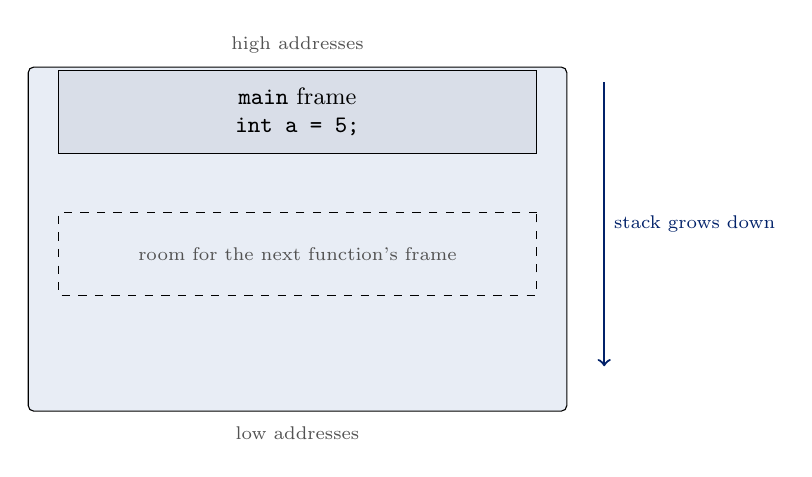
\begin{tikzpicture}[scale=0.95, every node/.style={scale=0.95}]
    \node[draw, fill=light-bg, minimum width=7.2cm, minimum height=4.6cm,
          rounded corners=2pt] at (0,-1.5) {};
    \node[font=\scriptsize, text=neutral] at (0,1.1) {high addresses};
    \node[draw, fill=primary-blue!15, minimum width=6.4cm, minimum height=1.1cm,
          align=center, font=\small] at (0,0.2)
          {\texttt{main} frame\\ \texttt{int a = 5;}};
    \node[draw, dashed, minimum width=6.4cm, minimum height=1.1cm,
          align=center, font=\scriptsize, text=neutral] at (0,-1.7)
          {room for the next function's frame};
    \draw[->, thick, color=primary-blue] (4.1,0.6) -- (4.1,-3.2)
      node[midway, right, font=\scriptsize] {stack grows down};
    \node[font=\scriptsize, text=neutral] at (0,-4.1) {low addresses};
  \end{tikzpicture}
  \caption{Stack growth, Step 1: \texttt{main} starts, its frame is created
  holding \texttt{int a = 5;}. The stack grows \emph{downward}.}
  \label{fig:stack1}
\end{figure}

\begin{example}[Stack growth, Step 2: \texttt{add} is called]
The call \texttt{add(x=5, y=3)} pushes a \emph{second} frame just below \texttt{main}'s, holding the parameters and \texttt{int s = x + y;} $= 8$ (Figure~\ref{fig:stack2}). Every new function call pushes a new frame just below the current one, so each new frame sits at a \key{lower} address than the frame above it.
\end{example}

\begin{figure}[h]
  \centering
  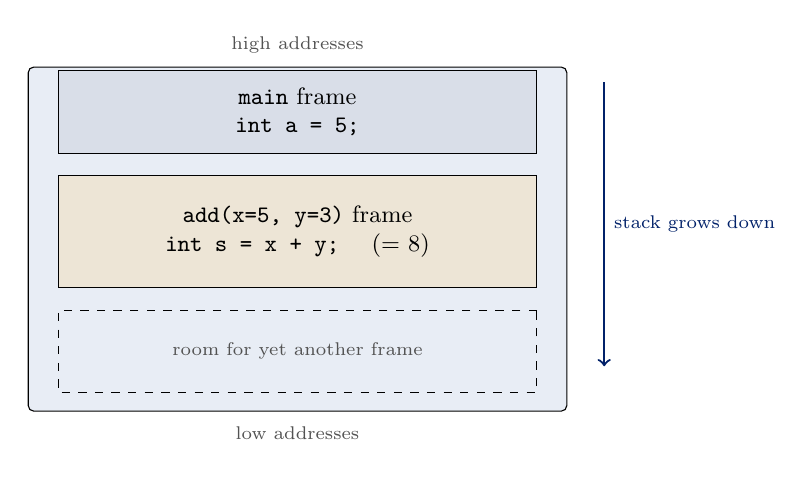
\begin{tikzpicture}[scale=0.95, every node/.style={scale=0.95}]
    \node[draw, fill=light-bg, minimum width=7.2cm, minimum height=4.6cm,
          rounded corners=2pt] at (0,-1.5) {};
    \node[font=\scriptsize, text=neutral] at (0,1.1) {high addresses};
    \node[draw, fill=primary-blue!15, minimum width=6.4cm, minimum height=1.1cm,
          align=center, font=\small] at (0,0.2)
          {\texttt{main} frame\\ \texttt{int a = 5;}};
    \node[draw, fill=primary-gold!25, minimum width=6.4cm, minimum height=1.5cm,
          align=center, font=\small] at (0,-1.4)
          {\texttt{add(x=5, y=3)} frame\\ \texttt{int s = x + y;} \quad (= 8)};
    \node[draw, dashed, minimum width=6.4cm, minimum height=1.1cm,
          align=center, font=\scriptsize, text=neutral] at (0,-3.0)
          {room for yet another frame};
    \draw[->, thick, color=primary-blue] (4.1,0.6) -- (4.1,-3.2)
      node[midway, right, font=\scriptsize] {stack grows down};
    \node[font=\scriptsize, text=neutral] at (0,-4.1) {low addresses};
  \end{tikzpicture}
  \caption{Stack growth, Step 2: the call to \texttt{add} pushes a second
  frame at a lower address than \texttt{main}'s.}
  \label{fig:stack2}
\end{figure}

\begin{example}[Stack growth, Step 3: \texttt{add} returns]
When \texttt{add} returns, its frame is popped --- it no longer exists, and its memory is available again (Figure~\ref{fig:stack3}). The answer \texttt{8} is copied back into \texttt{main}'s frame as \texttt{int s = 8;}. The stack has returned to its Step~1 shape.
\end{example}

\begin{figure}[h]
  \centering
  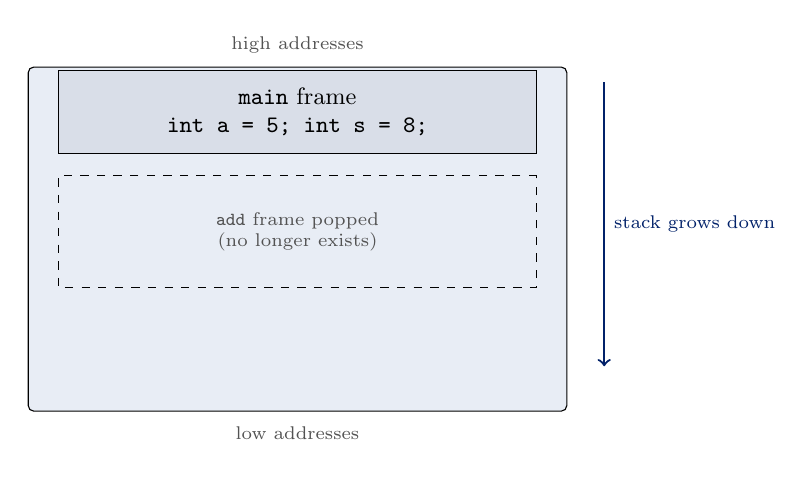
\begin{tikzpicture}[scale=0.95, every node/.style={scale=0.95}]
    \node[draw, fill=light-bg, minimum width=7.2cm, minimum height=4.6cm,
          rounded corners=2pt] at (0,-1.5) {};
    \node[font=\scriptsize, text=neutral] at (0,1.1) {high addresses};
    \node[draw, fill=primary-blue!15, minimum width=6.4cm, minimum height=1.1cm,
          align=center, font=\small] at (0,0.2)
          {\texttt{main} frame\\ \texttt{int a = 5; int s = 8;}};
    \node[draw, dashed, minimum width=6.4cm, minimum height=1.5cm,
          align=center, font=\scriptsize, text=neutral] at (0,-1.4)
          {\texttt{add} frame popped\\ (no longer exists)};
    \draw[->, thick, color=primary-blue] (4.1,0.6) -- (4.1,-3.2)
      node[midway, right, font=\scriptsize] {stack grows down};
    \node[font=\scriptsize, text=neutral] at (0,-4.1) {low addresses};
  \end{tikzpicture}
  \caption{Stack growth, Step 3: \texttt{add} returns, its frame is popped,
  \texttt{8} is copied back into \texttt{main}'s frame.}
  \label{fig:stack3}
\end{figure}

\textbf{Board: live stack trace (interactive, distinct instance 1).} Draw the empty board frame ahead of time. Ask one student to ``call'' \texttt{add} by walking to the board and drawing a new frame below \texttt{main}'s, labelling its contents; ask a second student to ``return'' by erasing that frame and writing \texttt{s = 8} into \texttt{main}'s. Ask mid-way: \emph{``where does the next frame go --- higher or lower address?''} (Lower --- the stack grows down.) Two volunteers, three steps, the whole class watches the stack grow and shrink.

\textbf{Board: distinct instance 2 (prediction trap).} Pose a different pair: \texttt{main} holds \texttt{int n = 3;} and calls \texttt{doubleIt(n)} whose local is \texttt{int d = 2*n;}. Ask the class to draw the two-frame picture \emph{before} you do, including which region is the higher address. Reveal after a show of hands. This is a genuinely different pair of functions from the deck's \texttt{main}/\texttt{add} example, so it exercises the same skill without being a restate.

\begin{teachingaside}
The recurring error here is treating the stack as ``a magic box that grows.'' The fix is the low-address/high-address labels drawn every time --- \emph{directions} (heap up, stack down) get fixed once and reused for 12 weeks; vary them once and you silently break a later diagram (Weeks 6--7, 11 all assume this orientation). Also be explicit that \emph{automatic} means ``the program manages it with zero instructions from you,'' not ``I don't have to think about it'' --- students conflate the two, and the conflation is exactly wrong once pointers into stack frames enter the picture (a dangling-pointer preview worth flagging even though the deck saves the term for the heap).
\end{teachingaside}

\subsection{Why the stack is not enough}

State the requirement the stack cannot meet: the user enters the record count only after the program runs, and we may need 3 records today, 300 tomorrow. The stack decides frame sizes at compile time and discards locals on return --- it fails on \emph{size} and on \emph{lifetime} simultaneously.

\textbf{Board: the guessing trap.} Write \texttt{int a[1000000];} and ask: ``when is this wasteful, and when does it still fail?'' (Wasteful when the actual count is small; fails outright the moment the real count exceeds a million --- guessing rescues nothing.) This reuses Wirth's p.111 argument without the formalism: a variable-sized structure ``cannot be assigned a fixed amount of storage,'' so allocation must happen \emph{when the data comes into existence} \cite{Wirth2004_algorithms_data_structures}, not at compile time.

\textbf{Board: the live prediction (distinct instance).} Put the two declarations on the board:
\begin{center}
\texttt{int score = 80;} \quad vs.\quad \texttt{int *p = malloc(sizeof(int));}
\end{center}
Ask: \emph{``which variable can outlive the function that created it?''} Let votes land before revealing. Answer: the \emph{block}, not the variable that names it --- the pointer is only the handle. Do not reveal \texttt{malloc} detail yet; you have told them the call exists, and that gap is the hook into the next two sections.

\section{Pointers: The Handle on Memory}
\label{sec:pointers}

\textbf{Read alongside:} Wirth, \S4.2, p.111 --- the dynamic-allocation argument and the address-as-handle picture.

\begin{definitionbox}{Pointer}
A variable that stores an address. Its type records what kind of object resides at that address \cite{Wirth2004_algorithms_data_structures}.
\end{definitionbox}

The contrast to draw explicitly: an ordinary variable stores a value such as \texttt{80}; a pointer stores a \emph{place}. \texttt{int *p;} means ``\texttt{p} can point to an \texttt{int}.'' Every pointer is a handle, never the data itself --- this is the single sentence students most need internalized before Section~\ref{sec:heap} makes it operational.

\begin{figure}[h]
  \centering
  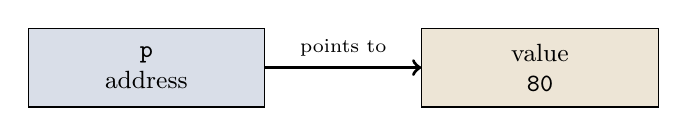
\begin{tikzpicture}[every node/.style={font=\small}]
    \node[draw, fill=primary-blue!15, minimum width=3.0cm, minimum height=1cm,
      align=center]
      (p) at (-2.5,0) {\texttt{p}\\address};
    \node[draw, fill=primary-gold!25, minimum width=3.0cm, minimum height=1cm,
      align=center]
      (x) at (2.5,0) {value\\\texttt{80}};
    \draw[->, very thick] (p.east) -- (x.west)
      node[midway, above, font=\scriptsize] {points to};
  \end{tikzpicture}
  \caption{A pointer picture: \texttt{p} holds an address; the value
  \texttt{80} lives at that address.}
  \label{fig:pointer-picture}
\end{figure}

\textbf{Board: box-and-arrow build order (distinct instance 1).} Draw the two boxes first, empty; write \texttt{80} in the right-hand box; only then draw the arrow, and label it ``points to'' last. Ask before drawing the arrow: \emph{``what does \texttt{p} contain --- the \texttt{80}, or the address?''} (The address.) The order matters pedagogically: drawing the arrow last mirrors the fact that the pointer's whole job \emph{is} the arrow, not the boxes.

\subsection{Pointers reach structures, and stop cleanly}

Introduce the two-field node, the building block for most of the term:
\begin{verbatim}
struct node {
  int data;
  struct node *next;
};
\end{verbatim}
\texttt{data} stores the value; \texttt{next} stores the address of \emph{another} node, or \texttt{NULL} if there is none. Establish the arrow field-access now, since the deck uses it from the first \texttt{malloc} example onward: \texttt{p->data} reads the \texttt{data} field of the node \texttt{p} points at.

\begin{definitionbox}{\texttt{NULL}}
The address value meaning ``points at nothing.'' Reading through it is undefined behaviour --- in practice, a crash.
\end{definitionbox}

\textbf{Board: node-picture drill (distinct instance 2, interactive).} Draw three boxes --- \texttt{head} at the left, then node~1 and node~2, each split into \texttt{data}/\texttt{next}. Ask the class to draw the arrows so \texttt{head} points at node~1, node~1's \texttt{next} points at node~2, and node~2's \texttt{next} is written \texttt{NULL}. Then erase the middle arrow and ask: \emph{``what happens to node~2 now?''} Answer: reachable no longer --- a preview of how a leak/dangling situation begins, even though the vocabulary is not introduced until Section~\ref{sec:heap-return}.

\textbf{Board: distinct instance --- extend the chain.} Ask the class to add a third node and mark where the chain terminates, then give the one-line meaning of \texttt{struct node *head = NULL;} (``the list is empty''). Two arrows and one \texttt{NULL} is a cheap repeat that fixes the convention (\texttt{head} as the list handle) before Week 6 needs it for real.

\begin{teachingaside}
Students arriving from an earlier course will write \texttt{(*p).data} and resist \texttt{p->data} as ``sugar.'' Hold the line: the course standard is \texttt{->} everywhere, per the notation registry, and \texttt{(*p).data} --- while correct C --- is noise this course does not use. Expect the ``is a pointer just a number?'' question too: yes, an address is a number, but the pointer's \emph{type} records what kind of object lives there, which is exactly why \texttt{int *} and \texttt{struct node *} are different types even though both ``just hold an address.''
\end{teachingaside}

\textbf{Live question:} ``if \texttt{p} points to a node and we set \texttt{p = NULL}, what happened to the node?'' (Nothing --- the node is untouched; only the pointer's value changed. This is the seed of the memory-leak idea, two sections early.)

\section{One Heap Block: Allocate, Use, Return}
\label{sec:heap}

The whole memory discipline of the course is three moves, applied to one block at a time: \good{request memory, use it, return it.} This section works through C's complete heap-allocation interface in the order a program actually needs it --- \texttt{malloc} and \texttt{sizeof} first, then the two allocation variants \texttt{calloc} and \texttt{realloc}, then the safe-node pattern, then the heap-growth picture, then \texttt{free} and the two beginner mistakes. Budget real time for all five calls; this is the largest section of the lecture and the one where board rehearsal pays off most.

\subsection{Requesting one integer: \texttt{malloc} and \texttt{sizeof}}
\label{sec:heap-detail}

\textbf{Read alongside:} Wirth, \S4.2, p.111.

State the pattern before explaining it:
\begin{verbatim}
int *p = malloc(sizeof(int));
if (p == NULL) return 1;
*p = 80;
\end{verbatim}
Three facts to narrate in order: \texttt{malloc(n)} requests \texttt{n} \emph{bytes} from the heap and returns their address, or \texttt{NULL} if the request fails; \texttt{sizeof(T)} is the compile-time size in bytes of type \texttt{T}, and it is what tells \texttt{malloc} how many bytes an \texttt{int} actually needs --- \texttt{malloc} never knows this on its own; and \texttt{p} stores the returned address, not the data. Emphasise explicitly: never count bytes by hand.

\textbf{Board: same pattern, distinct type (instance 1).} Walk the identical three lines for \texttt{double} instead of \texttt{int}: \texttt{double *d = malloc(sizeof(double)); if (d == NULL) return 1; *d = 3.5;}. Ask: \emph{``what changed between the \texttt{int} and \texttt{double} versions?''} Answer: only the type named in the declaration and inside \texttt{sizeof} --- the shape is identical. This ``one pattern, many types'' payoff is worth making explicit; it is the reason \texttt{sizeof} exists rather than a hand-counted constant.

\textbf{Board: live failure trace (instance 2).} Ask: \emph{``which line would fail if \texttt{p} is \texttt{NULL}?''} (Line three, the dereference \texttt{*p = 80;}.) If \texttt{malloc} returned \texttt{NULL}, an unguarded line three reads/writes through nothing --- a crash. The \texttt{if} guard turns line two into a controlled exit. Correct the habit live: never let a line touch a pointer that \emph{may} be \texttt{NULL} before it has been checked.

\begin{teachingaside}
The most common lab mistake this week is dropping \texttt{if (p == NULL)} ``because it never happens.'' The trace above is the fix: the dereference is unprotected, so an out-of-memory condition silently becomes a crash at a random later line, far from the actual bug. Also do not let students write \texttt{malloc(sizeof(8))} --- the argument to \texttt{sizeof} is a \emph{type} or an expression whose type is inferred, not a numeric literal that happens to look like a size.
\end{teachingaside}

\subsection{Zero-initialized memory: \texttt{calloc}}
\label{sec:calloc}

\begin{definitionbox}{\texttt{calloc}}
\texttt{calloc(n, size)} allocates space for \texttt{n} items of \texttt{size} bytes each, and sets \emph{every byte} of that space to \texttt{0}.
\end{definitionbox}
\begin{verbatim}
int *counts = calloc(5, sizeof(int));
if (counts == NULL) return 1;
\end{verbatim}
The request above asks for room for five integers, exactly as \texttt{malloc(5 * sizeof(int))} would, but with one added guarantee: \key{\texttt{calloc} zero-initializes; \texttt{malloc} does not.} That guarantee is the entire difference --- same style of request, same \texttt{NULL} check, different starting content.

Figure~\ref{fig:malloc-calloc} draws the contrast directly: two independent four-byte requests side by side, with no line connecting them --- they are unrelated blocks, shown together purely for comparison.

\begin{figure}[h]
  \centering
  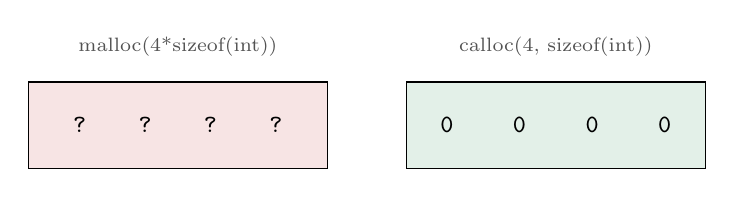
\begin{tikzpicture}[every node/.style={font=\small}]
    \node[font=\scriptsize, text=neutral] at (-2.4,1.0) {malloc(4*sizeof(int))};
    \node[draw, fill=negative!12, minimum width=3.8cm, minimum height=1.1cm,
      align=center, font=\ttfamily\small]
      (m) at (-2.4,0) {? \quad ? \quad ? \quad ?};
    \node[font=\scriptsize, text=neutral] at (2.4,1.0) {calloc(4, sizeof(int))};
    \node[draw, fill=positive!12, minimum width=3.8cm, minimum height=1.1cm,
      align=center, font=\ttfamily\small]
      (c) at (2.4,0) {0 \quad\; 0 \quad\; 0 \quad\; 0};
  \end{tikzpicture}
  \caption{\texttt{malloc} vs.\ \texttt{calloc}: \texttt{malloc} hands back
  four unspecified bytes (reading before writing is undefined behaviour);
  \texttt{calloc} hands back four bytes already zeroed.}
  \label{fig:malloc-calloc}
\end{figure}

\textbf{Board: walk the diagram, build order (instance 1).} Draw the left box first, unlabelled, and ask students to guess its contents before revealing the four \texttt{?} marks --- \emph{unspecified} means the bytes could be anything left over from a previous use of this memory, including garbage that happens to look valid. Only then draw the right box with its four zeros, and underline: same size request, only the starting content differs.

{\sloppy\textbf{Board: distinct instance 2.} Trace \texttt{struct point *pts =\allowbreak\ calloc(3,\allowbreak\ sizeof(struct point));} where \texttt{struct point} has two \texttt{int} fields \texttt{x} and \texttt{y}.\par} Ask: ``what are \texttt{pts[0].x} and \texttt{pts[1].y} immediately after this call, before any assignment?'' Answer: both \texttt{0} --- \texttt{calloc} zeroes every byte of the whole block, not just the first element, so every field of every struct in the array starts at zero. This generalizes the two-int example to the struct case students will actually use from Week 6 onward.

\begin{teachingaside}
Students routinely assume \texttt{malloc} also zero-initializes, usually because a test run ``happened to'' print zeros (freshly-mapped OS memory is often zero, which is an implementation accident, not a guarantee). The fix is insisting on the vocabulary distinction every time: \texttt{malloc}'s bytes are \emph{unspecified}, not \emph{zero} --- ``it worked when I tested it'' is not evidence of defined behaviour. \texttt{calloc} pays a small extra cost (writing the zeros) for the guarantee; that trade-off is worth stating explicitly so \texttt{calloc} does not look like a strictly-better free upgrade.
\end{teachingaside}

\textbf{Live question:} ``if you \texttt{malloc} an array and then read element \texttt{2} before writing to it, what can you say about the value you get back?'' (Nothing reliable --- it is unspecified, and reading it before writing is undefined behaviour in the strict sense, not just ``probably garbage.'')

\subsection{Resizing a block: \texttt{realloc}}
\label{sec:realloc}

\begin{definitionbox}{\texttt{realloc}}
\texttt{realloc(p, newsize)} resizes the block \texttt{p} points to, preserving its existing content up to the smaller of the old and new sizes. The block \key{may move} --- always keep the returned pointer.
\end{definitionbox}
\begin{verbatim}
int *bigger = realloc(p, 10 * sizeof(int));
if (bigger == NULL) return 1;  // p is still valid here
p = bigger;
\end{verbatim}
Two details in this idiom matter more than they look, and both are worth narrating explicitly rather than assuming students absorb them from reading the code: first, the check is against \texttt{bigger}, not \texttt{p} --- if \texttt{realloc} fails it returns \texttt{NULL} but leaves the \emph{original} block at \texttt{p} untouched, so overwriting \texttt{p} with a possibly-\texttt{NULL} result before checking would silently lose access to still-valid memory; second, \texttt{p} is reassigned to \texttt{bigger} only \emph{after} the check succeeds.

\begin{example}[Growing an array with \texttt{realloc}]
Start with \texttt{p = malloc(3 * sizeof(int))} holding \texttt{10 20 30}. Trace, one statement at a time, growing to five slots:
\begin{enumerate}
  \item \texttt{p = realloc(p, 5 * sizeof(int));} --- requests a block of five integers, built from the existing block at \texttt{p}.
  \item The first three ints (\texttt{10}, \texttt{20}, \texttt{30}) are \key{copied}, in order, by \texttt{realloc} itself --- the caller does not write this copy.
  \item The two new slots (index 3 and 4) are \key{unspecified} --- \texttt{realloc} does not zero new space; only \texttt{calloc} zeros space.
\end{enumerate}
If \texttt{realloc} returns \texttt{NULL}, the original block at \texttt{p} is untouched and still valid --- never overwrite \texttt{p} with the raw result before checking it, exactly as in the idiom above.
\end{example}

\textbf{Board: the growth trace, build order (instance 1).} Draw the original three-slot block first: \texttt{10 20 30}. Then draw a wider five-slot outline \emph{next to it} (not overwriting), and narrate the copy happening slot-by-slot: ``\texttt{realloc} copies \texttt{10} to slot 0, \texttt{20} to slot 1, \texttt{30} to slot 2 --- then leaves slots 3 and 4 blank.'' Only after the copy is drawn, mark slots 3--4 with \texttt{?} and ask: ``can we assume these are zero?'' (No --- only \texttt{calloc} guarantees that.)

\textbf{Board: distinct instance 2 --- \texttt{calloc} then \texttt{realloc} together.} This is the combination students will actually hit in code, so it is worth a full live trace: \texttt{p = calloc(3, sizeof(int));} then \texttt{q = realloc(p, 6 * sizeof(int));}. Ask the class to predict, before you draw: ``after both lines, what is in slots 0--2 of \texttt{q}, and what is in slots 3--5?'' Build the answer on the board: slots 0--2 were zeroed by \texttt{calloc} and then \emph{preserved} by \texttt{realloc}'s copy, so they remain \texttt{0}; slots 3--5 are the newly added space, which \texttt{realloc} never zeroes, so they are \key{unspecified} exactly like a fresh \texttt{malloc}'s bytes. The one-line summary worth writing on the board: \emph{``realloc preserves old content; it does not extend calloc's zero guarantee into new space.''}

\begin{teachingaside}
The two live-coding bugs to watch for: (1) writing \texttt{p = realloc(p, ...)} directly instead of assigning to a temporary first --- if this fails, \texttt{p} is now \texttt{NULL} and the original block's address is lost forever (a guaranteed leak, not just a missed error message); (2) assuming the two new slots in a grown block are zero because ``the old slots were zero'' (from a prior \texttt{calloc}) --- students generalize \texttt{calloc}'s guarantee to \texttt{realloc} because the two calls feel like siblings. They are not: only \texttt{calloc} zeroes, and only at the moment of that specific call.
\end{teachingaside}

\textbf{Live question:} ``if \texttt{realloc(p, newsize)} returns \texttt{NULL}, is the block at \texttt{p} still usable?'' (Yes --- explicitly, per the definition, the original block is untouched on failure. This is the fact the two-temporary idiom exists to protect.)

\subsection{Allocate a complete node: the safer engineering pattern}
\label{sec:node}

\begin{verbatim}
struct node *p = malloc(sizeof(struct node));
if (p == NULL) return 1;
p->data = 42;
p->next = NULL;
\end{verbatim}
Four properties to narrate, in the order the code enforces them: \texttt{sizeof(struct node)} asks for exactly one node's bytes, never a hand-counted \texttt{8} or \texttt{12} that breaks the moment a field is added or the code moves to another machine; the result is checked against \texttt{NULL} before anything touches the block; \texttt{p->data = 42;} sets the value field; \texttt{p->next = NULL;} makes the node's \emph{end} explicit. Initialising every field makes the node's state predictable --- an uninitialised field holds garbage, the same unspecified-content hazard from Section~\ref{sec:calloc}.

\textbf{Board: audit-the-node checklist (instance 1, interactive code review).} Write the four checks on the board and have the class \emph{vet a snippet you show}, not one you narrate:
\begin{enumerate}
  \item Was the allocation checked against \texttt{NULL}?
  \item Was every field initialised before the node was used?
  \item Is there exactly one clear owner responsible for \texttt{free(p)}?
  \item Can the program reach the node later, or has its pointer been lost?
\end{enumerate}
Show a deliberately broken variant --- omit the \texttt{NULL} check and \texttt{p->next = NULL;} --- and have students find both violations before you fix it live.

\textbf{Board: trace-before-run challenge (instance 2).} Put \texttt{int *p = malloc(sizeof(int)); *p = 80;} on the board and ask: \emph{``what is true after these lines?''} Build the answer as three separate facts, not one sentence: \texttt{p} contains an address; the heap block at that address contains \texttt{80}; the name \texttt{p} itself is \emph{not} the heap block --- they are two different objects in two different regions. Reuse Figure~\ref{fig:happened} as the shared reference picture, and pose the challenge live: \emph{``which line would fail if \texttt{p == NULL}?''} (The second line, the dereference.)

\begin{figure}[h]
  \centering
  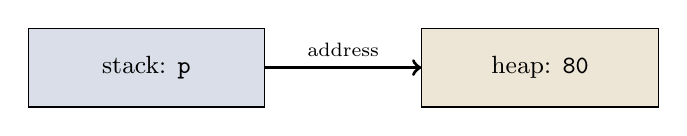
\begin{tikzpicture}[every node/.style={font=\small}]
    \node[draw, fill=primary-blue!15, minimum width=3cm, minimum height=1cm]
      (p) at (-2.5,0) {stack: \texttt{p}};
    \node[draw, fill=primary-gold!25, minimum width=3cm, minimum height=1cm]
      (box) at (2.5,0) {heap: \texttt{80}};
    \draw[->, very thick] (p.east) -- (box.west)
      node[midway, above, font=\scriptsize] {address};
  \end{tikzpicture}
  \caption{What happened: \texttt{p} lives on the stack and holds the address
  of a heap block containing \texttt{80}.}
  \label{fig:happened}
\end{figure}

\subsection{How the heap grows: a three-step story}
\label{sec:heap-growth}

The converse of the stack trace: the heap grows \emph{upward}, toward higher addresses. Three steps, mirroring the stack's three-step story exactly, so this is a good moment to have students notice the parallel structure rather than treat it as new material.

\begin{example}[Heap growth, Step 1: one \texttt{malloc} for three integers]
One \texttt{malloc} request with room for three integers grows the used heap upward, placing a block holding \texttt{10}, \texttt{20}, \texttt{30} (Figure~\ref{fig:heap1}). The block survives after the allocating function returns --- that is the heap's entire point, the direct payoff of Section~\ref{sec:memory}'s ``why the stack is not enough'' argument.
\end{example}

\begin{figure}[h]
  \centering
  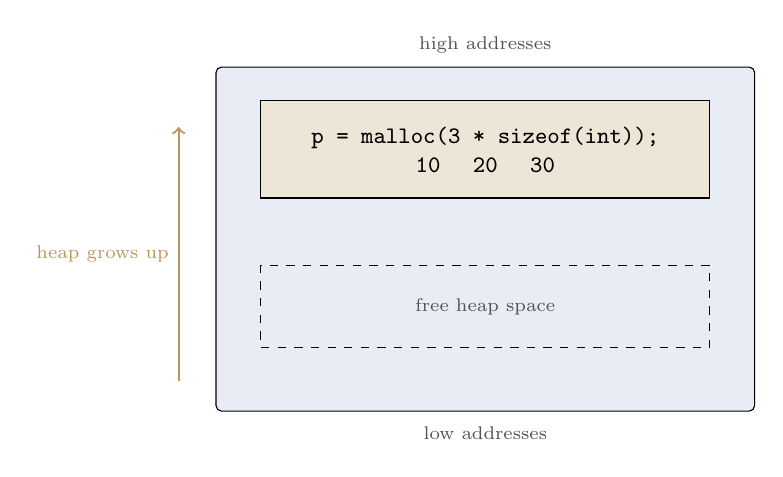
\begin{tikzpicture}[scale=0.95, every node/.style={scale=0.95}]
    \node[draw, fill=light-bg, minimum width=7.2cm, minimum height=4.6cm,
          rounded corners=2pt] at (0,-1.5) {};
    \node[font=\scriptsize, text=neutral] at (0,1.1) {high addresses};
    \node[draw, fill=primary-gold!25, minimum width=6.0cm, minimum height=1.3cm,
          align=center, font=\small] at (0,-0.3)
          {\texttt{p = malloc(3 * sizeof(int));}\\ \texttt{10} \quad \texttt{20} \quad \texttt{30}};
    \node[draw, dashed, minimum width=6.0cm, minimum height=1.1cm,
          align=center, font=\scriptsize, text=neutral] at (0,-2.4)
          {free heap space};
    \draw[->, thick, color=primary-gold] (-4.1,-3.4) -- (-4.1,0.0)
      node[midway, left, font=\scriptsize] {heap grows up};
    \node[font=\scriptsize, text=neutral] at (0,-4.1) {low addresses};
  \end{tikzpicture}
  \caption{Heap growth, Step 1: \texttt{malloc(3 * sizeof(int))} places one
  block holding \texttt{10}, \texttt{20}, \texttt{30}.}
  \label{fig:heap1}
\end{figure}

\begin{example}[Heap growth, Step 2: a second block]
The second request places \texttt{q}'s block at a \key{higher} address than \texttt{p}'s (Figure~\ref{fig:heap2}). Blocks are independent: each keeps its own data.
\end{example}

\begin{figure}[h]
  \centering
  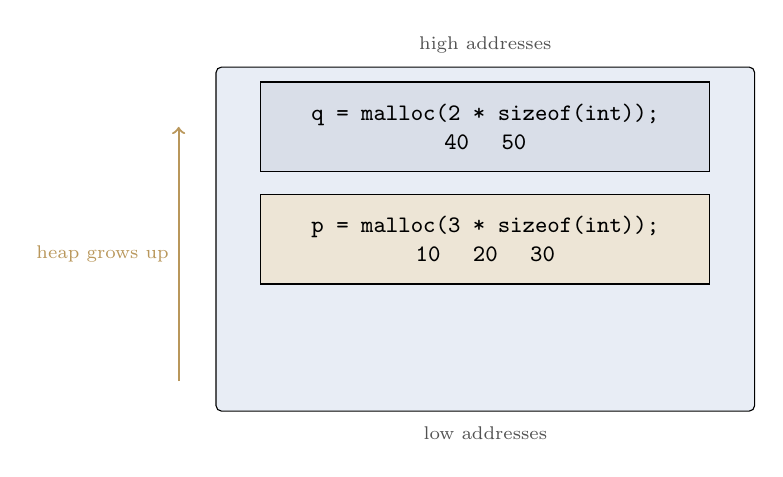
\begin{tikzpicture}[scale=0.95, every node/.style={scale=0.95}]
    \node[draw, fill=light-bg, minimum width=7.2cm, minimum height=4.6cm,
          rounded corners=2pt] at (0,-1.5) {};
    \node[font=\scriptsize, text=neutral] at (0,1.1) {high addresses};
    \node[draw, fill=primary-gold!25, minimum width=6.0cm, minimum height=1.2cm,
          align=center, font=\small] at (0,-1.5)
          {\texttt{p = malloc(3 * sizeof(int));}\\ \texttt{10} \quad \texttt{20} \quad \texttt{30}};
    \node[draw, fill=primary-blue!15, minimum width=6.0cm, minimum height=1.2cm,
          align=center, font=\small] at (0,0.0)
          {\texttt{q = malloc(2 * sizeof(int));}\\ \texttt{40} \quad \texttt{50}};
    \draw[->, thick, color=primary-gold] (-4.1,-3.4) -- (-4.1,0.0)
      node[midway, left, font=\scriptsize] {heap grows up};
    \node[font=\scriptsize, text=neutral] at (0,-4.1) {low addresses};
  \end{tikzpicture}
  \caption{Heap growth, Step 2: a second \texttt{malloc} places \texttt{q}'s
  block at a higher address; the two blocks are independent.}
  \label{fig:heap2}
\end{figure}

\begin{example}[Heap growth, Step 3: \texttt{free} returns a block]
\texttt{free(p)} gives \texttt{p}'s block back to the system (Figure~\ref{fig:heap3}); \texttt{q}'s block is untouched, and the used heap can shrink again.
\end{example}

\begin{figure}[h]
  \centering
  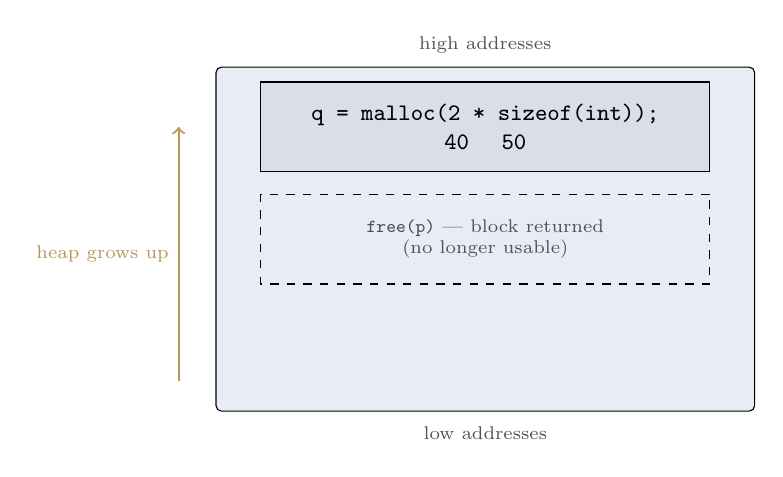
\begin{tikzpicture}[scale=0.95, every node/.style={scale=0.95}]
    \node[draw, fill=light-bg, minimum width=7.2cm, minimum height=4.6cm,
          rounded corners=2pt] at (0,-1.5) {};
    \node[font=\scriptsize, text=neutral] at (0,1.1) {high addresses};
    \node[draw, dashed, minimum width=6.0cm, minimum height=1.2cm,
          align=center, font=\scriptsize, text=neutral] at (0,-1.5)
          {\texttt{free(p)} --- block returned\\ (no longer usable)};
    \node[draw, fill=primary-blue!15, minimum width=6.0cm, minimum height=1.2cm,
          align=center, font=\small] at (0,0.0)
          {\texttt{q = malloc(2 * sizeof(int));}\\ \texttt{40} \quad \texttt{50}};
    \draw[->, thick, color=primary-gold] (-4.1,-3.4) -- (-4.1,0.0)
      node[midway, left, font=\scriptsize] {heap grows up};
    \node[font=\scriptsize, text=neutral] at (0,-4.1) {low addresses};
  \end{tikzpicture}
  \caption{Heap growth, Step 3: \texttt{free(p)} returns \texttt{p}'s block;
  \texttt{q}'s block is untouched.}
  \label{fig:heap3}
\end{figure}

\textbf{Board: heap growth trace (instance 1, interactive, three volunteers).} Draw the empty heap column. Volunteer 1 ``calls'' \texttt{malloc(3 * sizeof(int))} and draws the block holding \texttt{10 20 30} near the bottom; volunteer 2 ``calls'' \texttt{malloc(2 * sizeof(int))} for \texttt{q} and draws its block \emph{above} the first; volunteer 3 ``calls'' \texttt{free(p)} and shades the bottom region ``free again.'' The class watches the used heap grow up, then shrink from the bottom.

\begin{teachingaside}
The single most instructive contrast in the lecture is running the stack trace and the heap trace back to back and asking: \emph{``why opposite directions?''} Answer, if time permits (the deck says no more than this in Week~1): so the two regions can grow toward each other and share one contiguous free space without colliding --- the real layout of a process's address space. If you have covered both traces already, this is a two-sentence payoff; do not build a whole new example around it.
\end{teachingaside}

\textbf{Board: distinct instance 2 (prediction).} Cover Steps 2--3 and ask: \emph{``after \texttt{free(q)}, where does a new \texttt{malloc} of three integers land?''} Let guesses land, then reveal: exact placement is the allocator's choice; what matters is that freed space is \emph{reusable}, not its guessed address. This inoculates students against the common bug of hard-coding or reasoning about specific addresses.

\subsection{Returning the memory, and two beginner mistakes}
\label{sec:heap-return}

The return idiom is two lines that travel together, always:
\begin{verbatim}
free(p);
p = NULL;
\end{verbatim}
\texttt{free(p)} returns the heap block to the system; \texttt{p = NULL} makes the old pointer visibly empty so it cannot be mistakenly used as though the block still existed. This is the deck's summary line, and it is worth writing on the board verbatim: \good{request memory, use it, return it.} Every \texttt{malloc}/\texttt{calloc}/\texttt{realloc} block needs exactly one matching \texttt{free} --- the ``one'' matters as much as the ``matching.''

The two mistakes that violate this discipline:
\begin{itemize}
  \item \bad{Memory leak}: forget to call \texttt{free}; the block stays reserved forever, and if the only pointer to it is overwritten, nothing can ever reach it again. Nothing crashes --- the program quietly grows until it runs out of memory.
  \item \bad{Dangling pointer}: use a pointer after its block was freed. Reads return garbage; writes corrupt whatever now occupies that space.
\end{itemize}

\textbf{Board: the two mistakes side by side (instance 1, interactive clinical case).} Draw the heap with one live block, then:
\begin{enumerate}
  \item Sketch the \bad{leak}: erase the pointer variable's box while leaving the heap block drawn --- ask \emph{``who can still reach this block?''} (No one; it is unreachable but still reserved.)
  \item Sketch the \bad{dangling pointer}: shade the freed block ``free,'' but keep the pointer's arrow sharp and pointing at it --- ask \emph{``what does the arrow now point at?''} (Nothing usable; the block may already be handed to someone else.)
\end{enumerate}
The live habit to land: the owner is whoever frees. Ask a student to restate who owns the node from Section~\ref{sec:node}'s worked example.

\textbf{Board: distinct instance 2 --- the leak in a loop.} Show a program that allocates one node per loop iteration and never frees any of them. Trace the heap growing block after block with no volunteer ever shading anything ``free.'' Ask: \emph{``what eventually happens to this program?''} (It runs out of memory and dies --- nothing crashes on the first iteration, or the tenth, which is exactly why leaks are dangerous: the failure is delayed and looks unrelated to its cause.)

\begin{teachingaside}
Expect students to \texttt{free(p)} without setting \texttt{p = NULL}, then dereference the stale pointer in a later function and blame the compiler. Teach \texttt{free(p); p = NULL;} as \emph{one gesture}, not two independent lines --- say it as a single breath when narrating code. Also expect the ``I freed it but nothing bad happened'' shrug after a lab exercise: the bug is silent today and fatal on tomorrow's larger run, or on a different machine's allocator. That silence is the entire reason this discipline is taught as a habit rather than left to intuition.
\end{teachingaside}

\textbf{Live question:} ``between a memory leak and a dangling pointer, which one crashes your program \emph{today}, and which one might not crash it for a long time?'' (Dangling pointers often crash immediately or corrupt visibly; leaks are the slow, silent one --- a useful distinction for debugging intuition.)

\section{Simple Contracts: The ADT}
\label{sec:contracts}

\textbf{Read alongside:} Sedgewick \& Wayne, \S1.2, p.64; \S1.3, p.120; Karumanchi, Ch.~1, pp.18--19 (PDF); Aho--Hopcroft--Ullman, Ch.~1 (chapter-level).

We can now build a structure and reach it through a pointer. The remaining difficulty is describing one without drowning students in pointer mechanics every time --- which is exactly the payoff promised back in Section~\ref{sec:structured}'s live question: the data equivalent of ``a named, reusable block of logic'' is the ADT.

\begin{definitionbox}{Abstract data type (ADT)}
A description of what we can do with data, without saying how it is stored: a promise about operations \cite{Sedgewick2011_algorithms}.
\end{definitionbox}

Sedgewick \& Wayne state it as cleanly as anyone: a data type is ``a set of values and a set of operations on those values'' (p.64) \cite{Sedgewick2011_algorithms}. Karumanchi's treatment makes the same contract concrete by splitting it into two named parts: an ADT ``consists of two parts: 1. Declaration of data[;] 2. Declaration of operations'' (p.18, PDF) \cite{Karumanchi2017_data_structures_algorithms_made_easy}. The two framings agree exactly --- worth pointing out to students as evidence this is a stable idea, not one author's idiosyncratic phrasing.

\textbf{Board: the bag contract, write it first (instance 1).} Write, one line at a time:
\begin{enumerate}
  \item \texttt{insert(x)} --- put \texttt{x} into the bag.
  \item \texttt{member(x)} --- answer whether \texttt{x} is present.
  \item \texttt{size()} --- report how many items are present.
\end{enumerate}
Pause after writing all three and underline: \emph{the contract does not say whether the bag uses an array or a list.} That silence is the feature, not an omission --- say this explicitly, since students' instinct is to treat an unstated detail as a gap to fill in immediately.

\begin{figure}[h]
  \centering
  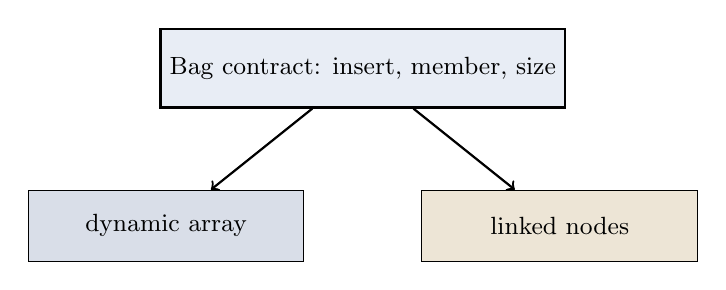
\begin{tikzpicture}[every node/.style={font=\small}]
    \node[draw, thick, fill=light-bg, minimum width=5cm, minimum height=1cm]
      (adt) at (0,2) {Bag contract: insert, member, size};
    \node[draw, fill=primary-blue!15, minimum width=3.5cm, minimum height=0.9cm]
      (array) at (-2.5,0) {dynamic array};
    \node[draw, fill=primary-gold!25, minimum width=3.5cm, minimum height=0.9cm]
      (list) at (2.5,0) {linked nodes};
    \draw[->, thick] (adt) -- (array);
    \draw[->, thick] (adt) -- (list);
  \end{tikzpicture}
  \caption{One contract, two implementations. Same operations, different
  internal arrangement; the caller's code does not change.}
  \label{fig:adt}
\end{figure}

\textbf{Board: one contract, two implementations (instance 2, interactive classify).} Draw the contract box first, alone, and only add the two implementation boxes below it afterward, connected by ``implements'' arrows (Figure~\ref{fig:adt}) --- the build order matters: contract first mirrors the course's own rule (state the contract before writing a line of the implementation). Then run the deck's classify drill live, by show of hands:
\begin{enumerate}
  \item ``\texttt{member(7)} answers yes or no.'' --- \good{contract}: what users can ask.
  \item ``The values are stored in an array.'' --- \bad{implementation}: how.
  \item ``\texttt{size()} reports the number of values.'' --- \good{contract}: what users can ask.
\end{enumerate}

\textbf{Board: distinct instance 3 (design question).} Pose a variant contract --- ``a queue of integers with \texttt{enqueue} and \texttt{dequeue}'' --- and ask which of the two implementation boxes the class \emph{guesses} is cheaper for \texttt{dequeue}. Either answer is pedagogically fine here; the point is that both \emph{could} implement it, which is exactly the abstract claim the bag example just made. Sedgewick \& Wayne's \S1.3 (p.120) frames bag/queue/stack as three collections differing only in which object is removed next --- worth a one-minute pointer for curious students.

\textbf{Board: the course roadmap, ADT by ADT.} List on the board: Linked Lists, Stacks, Queues, Priority Queues, Binary Trees, Hash Tables, Graphs --- the commonly used ADTs, in Karumanchi's phrasing (pp.18--19, PDF) \cite{Karumanchi2017_data_structures_algorithms_made_easy}. Point out this is not a random list: it is the Weeks~3--12 work-list, and every one of those weeks opens the same three-beat way this section just did --- ``What is a Stack?'', then ``Stack ADT'', \emph{then} implementation. Today's bag is the class's first rehearsal of a pattern the course repeats eight more times.

\begin{teachingaside}
Karumanchi2017 is a strong anchor for the \emph{shape} of the ADT idea and for this roadmap, but it is deliberately not cited anywhere in the stack, heap, or pointer sections above --- indexing (Step~0.5) confirmed it has zero coverage there of structured programming or of C's heap-allocation calls. When answering student questions live: cite Karumanchi2017 for ``what is an ADT'' and ``what's coming''; cite Wirth2004 for the C memory-management mechanics. Mixing the two up in front of the class is an easy, avoidable slip.
\end{teachingaside}

\begin{teachingaside}
The ADT section is where classes mentally check out unless it is \emph{used}. The classify drill is the anchor --- it forces the what-vs-how split out of each student rather than letting them nod along. Do not present the ADT as a vocabulary item; present it as a design decision, and preview explicitly that Weeks~3 and~7 implement the \emph{same} stack twice, over an array and then over linked nodes, so the choice becomes real rather than hypothetical. This is deliberately the lightest-weight theoretical point of the lecture, matching the intro-tier difficulty --- do not over-formalize it with axioms or algebraic laws; that is a later-course concern.
\end{teachingaside}

\textbf{Live question:} ``we said a function is a named, reusable block of logic, and today we've named the data equivalent an ADT. What's the one-sentence version of the parallel?'' (State the contract/interface before writing the implementation --- for functions \emph{and} for data, the exact same discipline, one level up.)

\section{Synthesis and Summary}

Close by returning to the three prediction boxes from Section~\ref{sec:act0}'s opening frame and filling them in together with the class: \emph{where} = the stack (short-lived locals) and the heap (run-time requests); \emph{how} = \texttt{malloc}/\texttt{sizeof}/\texttt{calloc}/\texttt{realloc} obtain a heap block and \texttt{free} returns it, all reached through a pointer handle; \emph{describe} = an ADT states operations before any implementation. The three boxes are the three of the four opening questions this Act answers with mechanism; question 1 (structuring logic) was answered by the Structured Programming Act itself, and its payoff --- ``the same discipline, reapplied to data'' --- is the sentence that ties the whole lecture together.

\textbf{Quick reference.} \emph{Stack:} automatic, scope-bound, grows down; each call pushes a frame, each return pops it. \emph{Heap:} run-time sized, lifetime-controlled by you, grows up; \texttt{malloc}/\texttt{calloc} obtain, \texttt{realloc} resizes, \texttt{free} returns, \texttt{NULL} means ``nothing.'' \emph{Pointer:} stores an address; \texttt{->} reads a field; never read through \texttt{NULL}. \emph{Allocation idiom:} \texttt{malloc}+\texttt{sizeof} for unspecified content, \texttt{calloc} for zero-initialized content, \texttt{realloc} to resize (never overwrite the old pointer before checking the result) $\rightarrow$ check \texttt{NULL} $\rightarrow$ initialise every field $\rightarrow$ use $\rightarrow$ \texttt{free} + set \texttt{NULL}. \emph{Two mistakes:} leak (never freed, silent) and dangling pointer (used after free, often loud); every allocation has exactly one owner. \emph{ADT:} operations stated without storage; a data structure is one implementation of the contract.

Set up Week 2's hook explicitly, tying back to Section~\ref{sec:act0}'s Sedgewick quote: we can now build two implementations of the same bag, but we have no way to say which is better --- only ``it felt fast,'' which Sedgewick's \S1.4 (p.172) already told us is too vague to answer precisely. Week 2 supplies the vocabulary --- $T(n)$, asymptotic classes, best/worst/average case --- to compare implementations without ever running either one.

\bibliographystyle{plain}
\bibliography{../../Bibliography_base}

\end{document}
